\chapter[Synchronous emplacement of the anorthosite xenolith-bearing Beaver River diabase and one of the largest lava flows on Earth][Beaver Bay Complex]{Synchronous emplacement of the anorthosite xenolith-bearing Beaver River diabase and one of the largest lava flows on Earth}

\let\thefootnote\relax\footnote{This chapter is published as a peer-reviewed manuscript: Zhang, Y., Swanson-Hysell, N.L., Schmitz, M.D., Miller Jr., J.D., and Avery, M.S., (2021), Synchronous emplacement of the anorthosite xenolith-bearing Beaver River diabase and one of the largest lava flows on Earth. Geochemistry, Geophysics, Geosystems. doi: \url{https://doi.org/10.1029/2021GC009909}.}

\section{Abstract}
New geochronologic and paleomagnetic data from the North American Midcontinent Rift (MCR) reveal the synchronous emplacement of the Beaver River diabase, the anorthosite xenoliths within it, and the Greenstone Flow --- one of the largest lava flows on Earth. A U-Pb zircon date of 1091.83 $\pm$ 0.21 Ma (2$\sigma$) from one of the anorthosite xenoliths is consistent with the anorthosite cumulate forming as part of the Midcontinent Rift and provides a maximum age constraint for the Beaver River diabase. Paired with the minimum age constraint of a cross-cutting Silver Bay intrusion (1091.61 $\pm$ 0.14 Ma; 2$\sigma$) these data tightly bracket the age of the Beaver River diabase to be 1091.7 $\pm$ 0.2 Ma (95\% CI), coeval with the eruption of the Greenstone Flow (1091.59 $\pm$ 0.27 Ma; 2$\sigma$) --- which is further supported by indistinguishable tilt-corrected paleomagnetic pole positions. Geochronological, paleomagnetic, mineralogical, and geochemical data are consistent with a hypothesis that the Beaver River diabase was the feeder system for the Greenstone Flow. The large areal extent of the intrusives and large estimated volume of the volcanics suggest that they represent a rapid and voluminous ca. 1092 Ma magmatic pulse near the end of the main stage of MCR magmatism.

\section{Introduction}

The North American Midcontinent Rift (MCR) is a ca. 1.1 Ga large igneous province for which there is excellent exposure of both the intrusive and extrusive components in the Lake Superior region (Fig. \ref{Chap_BBC_Geologic_map}). An exceptional feature within the Midcontinent Rift is the occurrence of large anorthosite xenoliths within a diabase sill and dike network known as the Beaver River diabase that outcrops in northeastern Minnesota, USA, as part of the Beaver Bay Complex (Fig. \ref{Chap_BBC_Geologic_map}). The anorthosite xenoliths range in size from centimeter-scale megacrysts to meter-scale, decimeter-scale and even $>$150 meter-scale blocks (Fig. \ref{fig:Chap_BBC_Field_photo}; \citealp{Morrison1983a, Grout1939a}). A particularly large anorthosite xenolith is exposed at Carlton Peak in the eastern Beaver Bay Complex with minimum dimensions of 180 $\times$ 240 meters (Fig. \ref{Chap_BBC_Geologic_map}, \ref{fig:Chap_BBC_Field_photo}; \citealp{Boerboom2006b}). In the southern Beaver Bay Complex, a large anorthosite xenolith near Corundum Point has dimensions of 180 $\times$ 230 meters while one exposed at Split Rock Point has dimensions of 180 $\times$ 260 meters \citep{Boerboom2004a}. To be able to accommodate such large xenoliths during magma ascent, the Beaver River diabase conduits must have been of at least the width of the anorthosite short axis diameters. Such wide conduits in these near-surface intrusions suggest high magma flux rates and make it likely that the magma extruded to the surface --- feeding voluminous lava flows.  

\begin{figure}[h!]
\noindent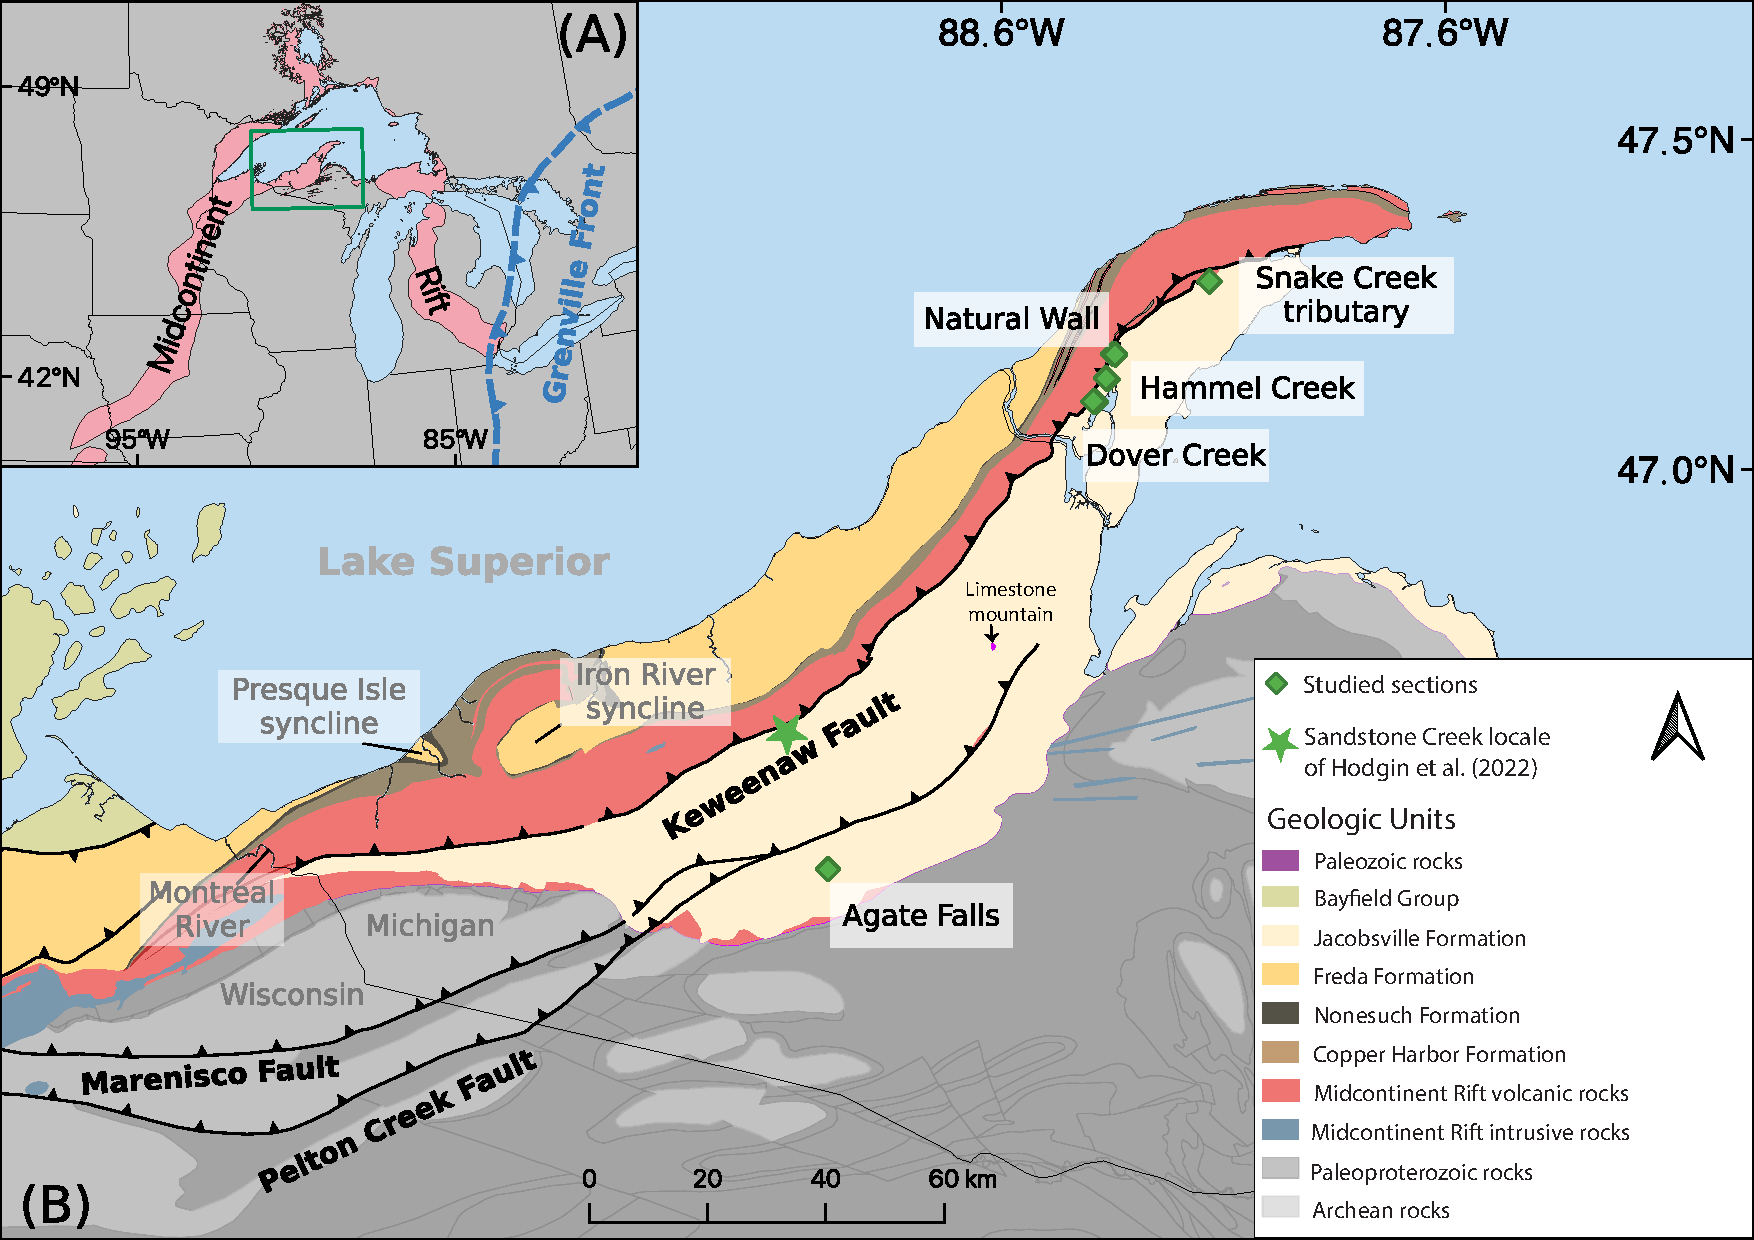
\includegraphics[width=0.85\textwidth]{figure/Zhang2021/Geologic_map.pdf}
\centering
\caption[Simplified geologic map of the Midcontinent Rift and regional maps of the Beaver Bay Complex]{\footnotesize{(A) Geologic map of exposures of Midcontinent Rift volcanics and intrusives in the western Lake Superior region. The Greenstone Flow (purple) of the Portage Lake Volcanics (red) outcrops throughout the Keweenaw Peninsula and Isle Royale. (B) Regional map of paleomagnetic and geochronologic sites in the southern Beaver Bay Complex (south BBC). Note that paleomagnetic site AX16 and geochronology sample MS99033 are from the same anorthosite xenolith. The geochronology sample numbers in (A) and (B) correspond to those in Fig. \ref{fig:BBC_geochron}. (C) Regional map of paleomagnetic sites in the eastern Beaver Bay Complex (east BBC). The xenolith at Carlton Peak is $>$100 meters in diameter. The younger Schroeder-Lutsen basalt of the North Shore Volcanic Group (NSVG) is lying unconformably atop the Beaver River diabase and other NSVG units. The nomenclature of the ``southern" and ``eastern" Beaver Bay Complex follows \cite{Miller1997a}. FTMD - Finland tectonomagmatic discontinuity, traced out by the dashed black line. Bedrock geology is from \cite{Miller2001a} and \cite{Jirsa2011a}.}}
\label{Chap_BBC_Geologic_map}
\end{figure}

\cite{Miller1997a} emphasized the composite nature of the Beaver River diabase network and Silver Bay intrusions (Fig. \ref{Chap_BBC_Geologic_map}), which are locally marked by abrupt transitions to progressively more evolved lithologies. Furthermore, \cite{Miller1997a} documented geochronologic, geochemical and structural evidence to support the notion that the diabase network may have served as principal feeder conduits to lava flows including parts of the Portage Lake Volcanics on the Keweenaw Peninsula and Isle Royale of Michigan (Fig. \ref{Chap_BBC_Geologic_map}). To more directly test this inferred intrusive-extrusive correlation, \cite{Doyle2016a} compared the mineralogical, textural, and geochemical attributes and the composite lithologic nature of the Beaver River diabase against those of the Greenstone Flow, the largest lava flow within the Midcontinent Rift and one of the largest lava flows on Earth (Fig. \ref{fig:lava_flow_rank}). \cite{Doyle2016a} documented remarkable similarities in petrography, mineral chemistry, whole rock geochemistry, and interpreted lithologic zonation between the Beaver River diabase intrusions in northern Minnesota and the Greenstone Flow on both Isle Royale and Keweenaw Peninsula. Based on the interpreted feeder system being in northern Minnesota, \cite{Doyle2016a} estimated the full areal extent of the Greenstone Flow to be $\sim$20000 km$^2$ and its volume to be between 2000 and 6000 km$^3$ (Fig. \ref{fig:lava_flow_rank}). 

A comagmatic relationship between the Beaver River diabase and the Greenstone Flow is consistent with the similar $^{207}$Pb/$^{206}$Pb dates developed from a granophyric ferrogabbro within the Beaver Bay Complex (1095.8 $\pm$ 1.2 Ma; \citealp{Paces1993a}) and the Greenstone Flow (1094.0 $\pm$ 1.5 Ma; \citealp{Davis1990a}). The relatively large uncertainties provided by the existing $^{207}$Pb/$^{206}$Pb geochronology provide less precise estimates of the temporal relationships between these rapid events than is possible with modern methods. Modern-day U-Pb geochronology techniques for chemical abrasion isotope dilution-thermal ionization mass spectrometry (CA-ID-TIMS) allow high-precision $^{206}$Pb/$^{238}$U dates to be developed from chemically abraded zircon crystals \citep{Mattinson2005a}. Studies utilizing these methods on Midcontinent Rift volcanic and intrusive rocks have shown that the analytical uncertainties on weighted mean $^{206}$Pb/$^{238}$U dates of multiple chemically abraded single zircons can be $\sim$200 kyr, an order of magnitude smaller than previous dates that are based exclusively on the $^{207}$Pb/$^{206}$Pb system \citep{Fairchild2017a, Swanson-Hysell2019a, Swanson-Hysell2021a}. These $^{206}$Pb/$^{238}$U dates are also considered to be more accurate than systematically older $^{207}$Pb/$^{206}$Pb dates \citep{Schoene2006a}. Such $^{206}$Pb/$^{238}$U dates indicate that the massive Layered Series and Anorthositic Series rocks of the Duluth Complex were emplaced in $\sim$500 kyr ca. 1096 Ma \citep{Swanson-Hysell2021a}.  

In this work, we use a new $^{206}$Pb/$^{238}$U zircon date for an anorthosite xenolith hosted within the Beaver River diabase, in conjunction with $^{206}$Pb/$^{238}$U dates from a Silver Bay intrusion and the Greenstone Flow (Fig. \ref{Chap_BBC_Geologic_map}; \citealp{Fairchild2017a}), to evaluate the timing of emplacement of the Beaver River diabase, and the hypothesized intrusive-extrusive correlation between the Beaver River diabase and the Greenstone Flow.

Paleomagnetic data can also provide chronological constraints on rock units. Laurentia experienced a period of rapid latitudinal plate motion during rift development \citep{Swanson-Hysell2009a}. A synthesized apparent polar wander path (APWP) based on the Midcontinent Rift volcanic rocks indicates that motion exceeded 20 cm/yr \citep{Swanson-Hysell2019a}, faster than the maximum speed of India of $\sim$17 cm/yr during the Cenozoic \citep{Hinsbergen2011a}. This motion resulted in significant differences in pole positions recorded by Midcontinent Rift rocks that were emplaced a few million years apart \citep{Swanson-Hysell2019a}. In this study, we present paleomagnetic data from the anorthosite xenoliths and the host Beaver River diabase. Data from the xenoliths give equivalent directions to the host diabase (Figs. \ref{fig:Demag}, \ref{fig:Direction_pairs}), indicating that they were heated above the Curie temperature of magnetite and acquired a thermal remanent magnetization when they cooled within the diabase. This thermal history is consistent with thermal diffusion modeling of the xenoliths (Fig. \ref{fig:thermal_history_model}). The paleomagnetic data can be compared to data from the Greenstone Flow to further test the hypothesis that they are synchronous. The resulting paleomagnetic pole positions can also be compared to the synthesized Laurentia APWP to obtain chronological constraints (Fig. \ref{fig:Direction_pairs}).

Here, by integrating the geochronologic and paleomagnetic perspectives with previous lithologic and geochemical analyses \citep{Miller1997a, Doyle2016a}, we show that these data are consistent with the Beaver River diabase network acting as the feeder system for the Greenstone Flow of the Portage lake Volcanics. Alternatively, they could both be the distinct manifestations of magmatism from a similar source. Regardless, their shared geochemical signatures and the inference of giant magma conduits that transported large anorthosite xenoliths characterize a period of ca. 1092 Ma voluminous magmatic activity (based on $^{206}$Pb/$^{238}$U zircon dates; Fig. \ref{Chap_BBC_Geologic_map}).

\section{Geologic Setting}

\subsection{Beaver Bay Complex and Related Rocks of NE Minnesota}

\begin{figure}[h!]
\centering
\noindent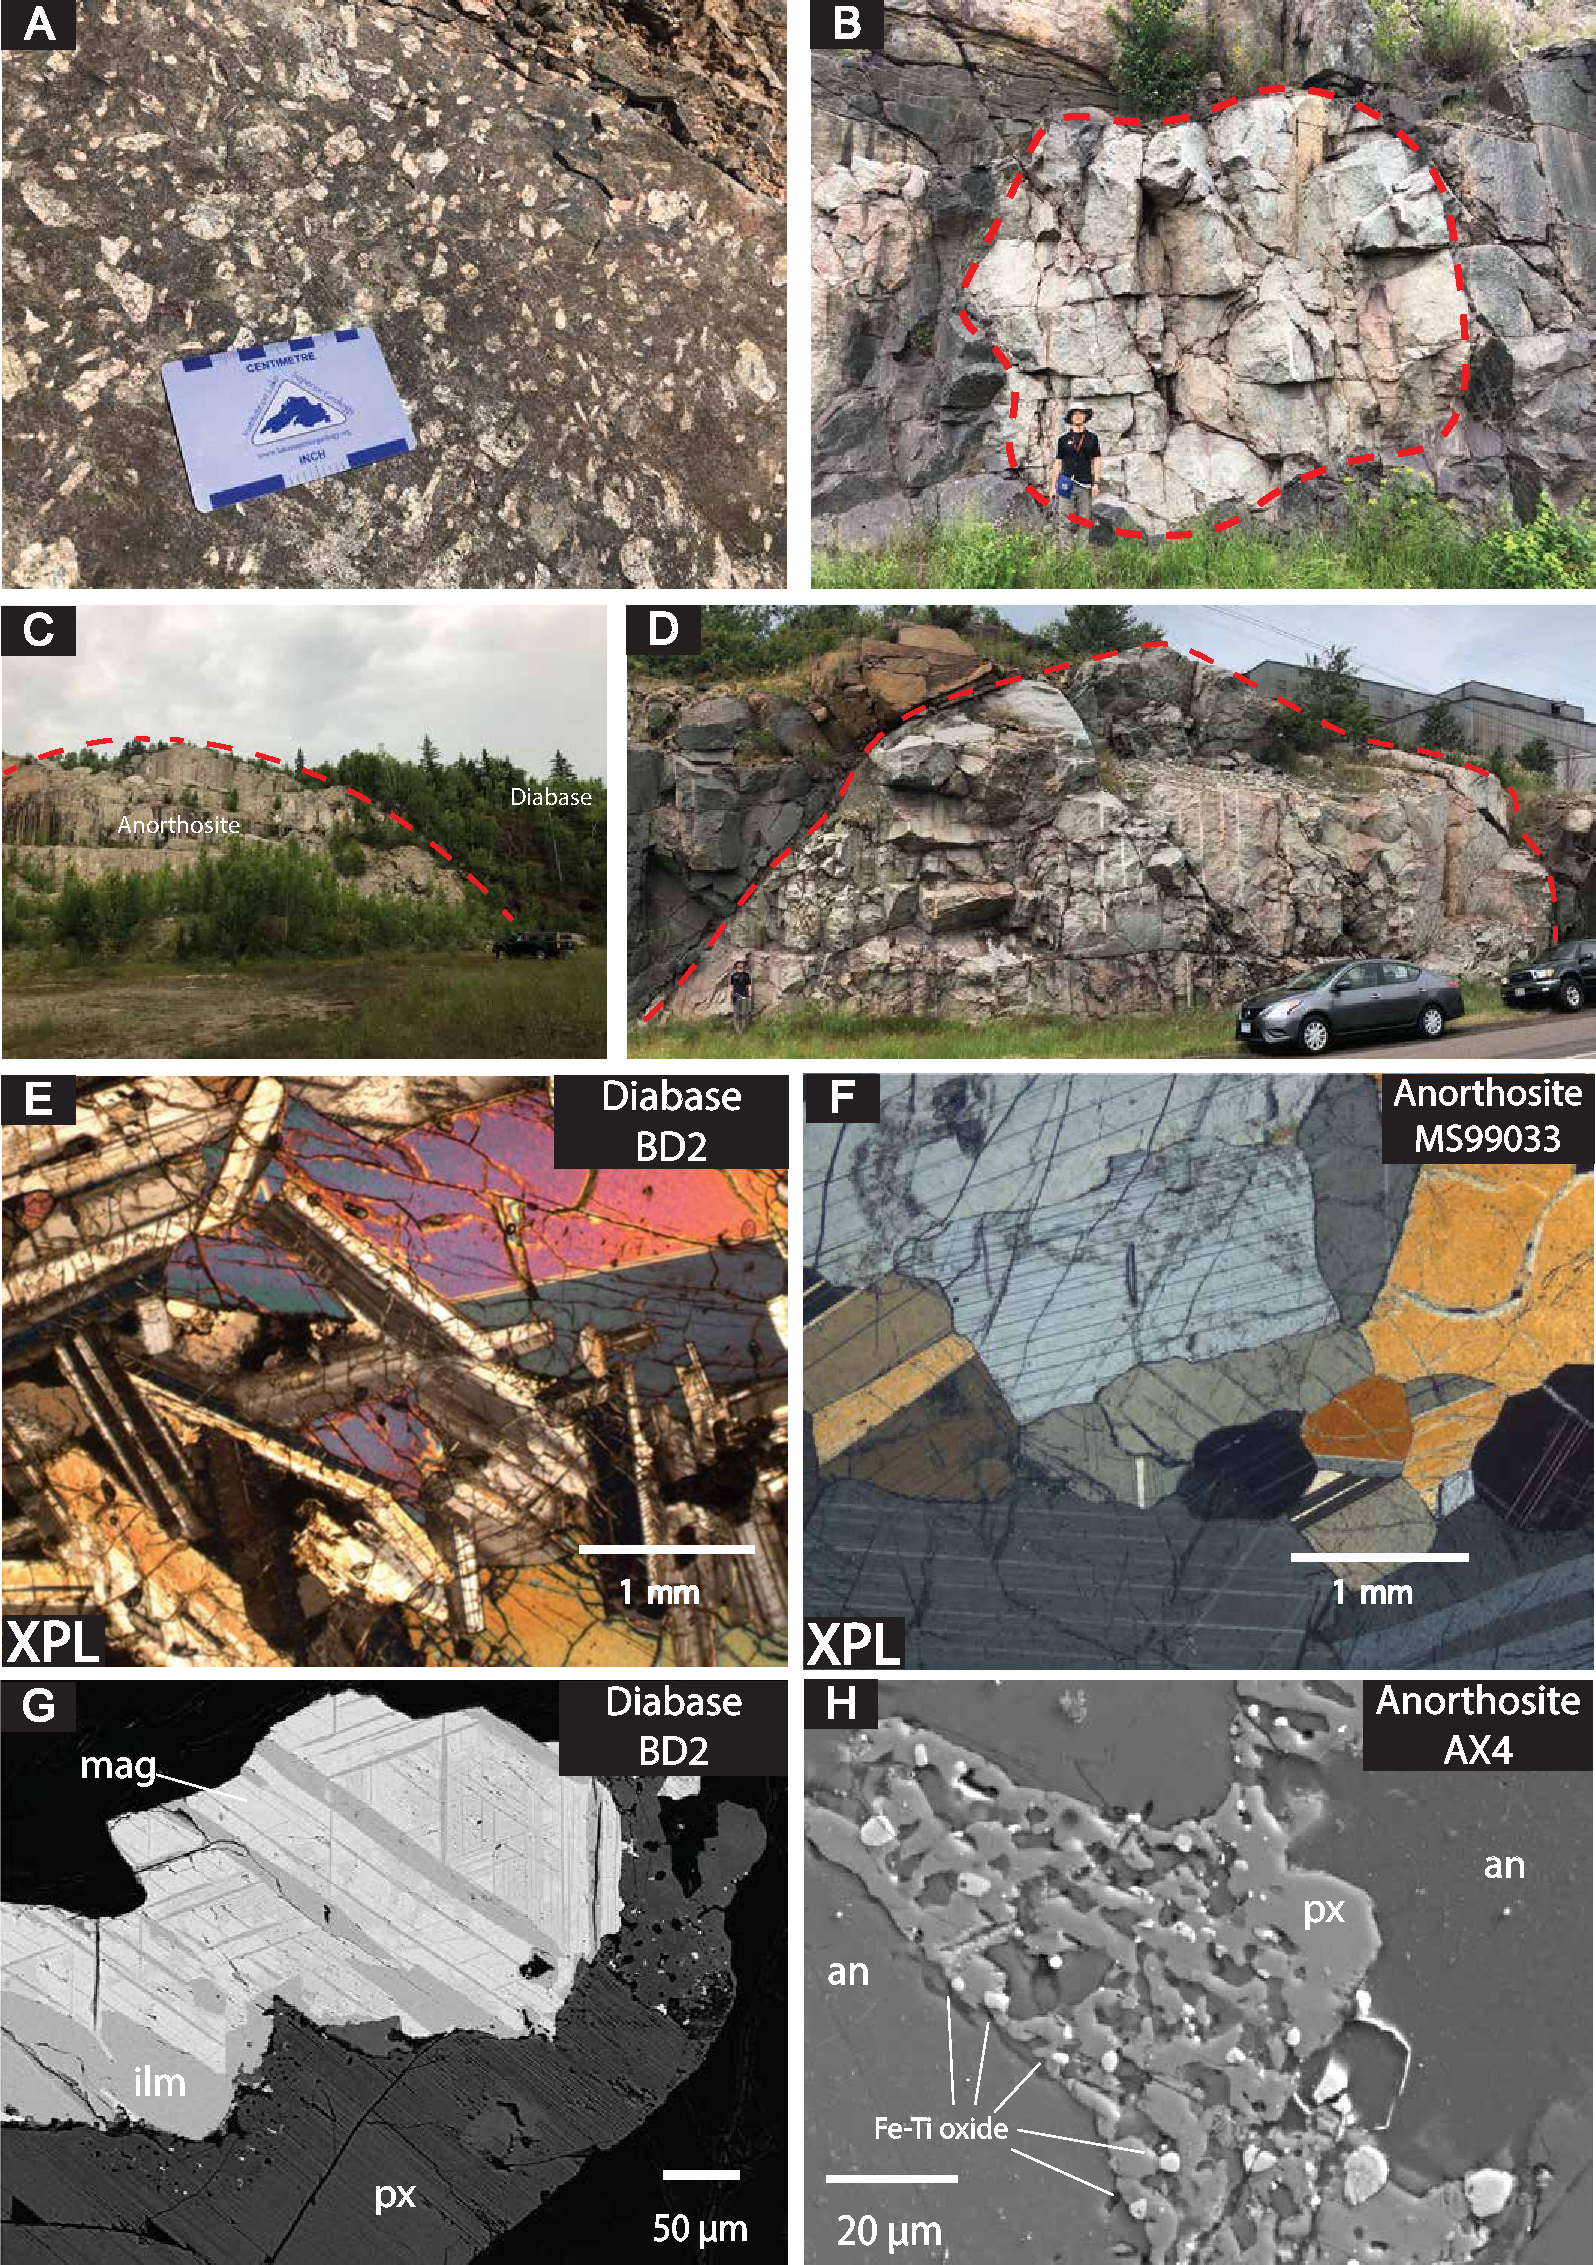
\includegraphics[width=0.62\textwidth]{figure/Zhang2021/Field_photo.pdf}
\caption[Field photographs and petrographic images of the Beaver River diabase and the anorthosite xenoliths]{\footnotesize{Field photographs and petrographic images of the Beaver River diabase and the anorthosite xenoliths within it. (A) Centimeter-sized plagioclase megacrysts in the diabase. (B) Rounded anorthosite xenolith with a diameter of $\sim$7 meters fully enclosed within the diabase. (C) Exposure of a giant Carlton Peak anorthosite with a diameter $>$100 m. (D) 27.5 m diameter anorthosite xenolith sampled as paleomagnetic site AX16 and geochronology sample MS99033. (E) Cross polarized (XPL) image of the subophitic texture of diabase at site BD2 (pyroxene partially enclosing plagioclase). (F) XPL image of anorthosite geochronology sample MS99033. Plagioclase crystals exhibit both granoblastic texture and interlocking lath fabrics. (G) Backscattered electron (BSE) image of a large Fe-Ti oxide with titanomagnetite-ilmenite lamellae in Beaver River diabase site BD2. (H) BSE image of micron-sized Fe-Ti oxides exsolved from pyroxene between plagioclase crystals in anorthosite xenolith site AX4. an-plagioclase with $\sim$70\% anorthite; ilm-ilmenite; mag-magnetite; px-pyroxene.}}
\label{fig:Chap_BBC_Field_photo}
\end{figure}

The North American Midcontinent Rift (MCR) is a failed intracontinental rift where protracted magmatic activity lasted from ca. 1109 Ma to ca. 1084 Ma \citep{Swanson-Hysell2019a}. Midcontinent Rift rocks extensively outcrop in today's Lake Superior region, with the total extent traceable by arcuate magnetic and gravity anomalies that extend to the southwest to Kansas, and to the southeast, to southern Michigan \citep{Hinze2020a}. Previous studies have divided magmatic activity in the rift into four stages based on interpreted changes in relative magmatic volume and the nature of magmatism: early ($\sim$1109--1104 Ma), latent ($\sim$1104--1098 Ma), main ($\sim$1098--1090 Ma) and late ($\sim$1090--1083 Ma) \citep{Vervoort2007a, Heaman2007a, Miller2013a}. In northeastern Minnesota, the Early Gabbro Series and the Felsic Series rocks of the Duluth Complex and reversed-polarity lavas of the lower North Shore Volcanic Group were emplaced during the early stage. The more voluminous Duluth Complex Layered Series and the plagioclase-rich Anorthositic Series, together with an associated $\sim$8 km thick extrusive volcanic sequences of the North Shore Volcanic Group (NSVG), were rapidly emplaced about 10 myr later at ca. 1096 Ma during the main stage \citep{Paces1993a, Swanson-Hysell2021a}. 

The Beaver Bay Complex, which sits stratigraphically above the Duluth Complex, is another intrusive complex that resulted from main stage magmatism. The exposed area of the Beaver Bay Complex is $\sim$1000 km\textsuperscript{2} where it has been mapped along the northwestern shore of Lake Superior in northeastern Minnesota (Fig. \ref{Chap_BBC_Geologic_map}). The Beaver Bay Complex is a multi-phase, composite intrusive complex that intrudes parts of the NSVG (Fig. \ref{Chap_BBC_Geologic_map}; \citealp{Miller1997a, Swanson-Hysell2021a}). Distinct from the deep plutonic intrusions of the Duluth Complex, the majority of the Beaver Bay Complex is formed of hypabyssal intrusions that were emplaced as dikes and sills at shallow depths \citep{Miller1997a}. Most of the Beaver Bay Complex intrusions are dioritic to gabbroic in composition \citep{Miller1997a}. The main lithology of the Beaver River diabase dikes and sills network within the Beaver Bay Complex is an ophitic olivine gabbro (Fig. \ref{fig:Chap_BBC_Field_photo}), but in wider areas of dikes and the upper parts of thick sills, this rock type can abruptly transition into intergranular olivine oxide gabbro, then into subprismatic (and commonly foliated) ferrogabbro, and finally into granophyric monzodiorite. The more evolved and later emplaced components of the Beaver River diabase network are commonly distinguished as the Silver Bay intrusions in the southern Beaver Bay Complex (Fig. \ref{Chap_BBC_Geologic_map}). Overall being intermediate in composition, the Silver Bay intrusions lithologies range from ophitic olivine gabbro to ferrogranite \citep{Shank1989a}. Field mapping by \cite{Miller1994a} found intrusive relationships between the Silver Bay intrusions and the Beaver River diabase. Angular inclusions of the host Beaver River diabase within marginal zones of the Silver Bay intrusions led \cite{Miller1997a} to interpret that the Silver Bay intrusions intruded after the diabase crystallized.


\begin{figure}[h!]
\noindent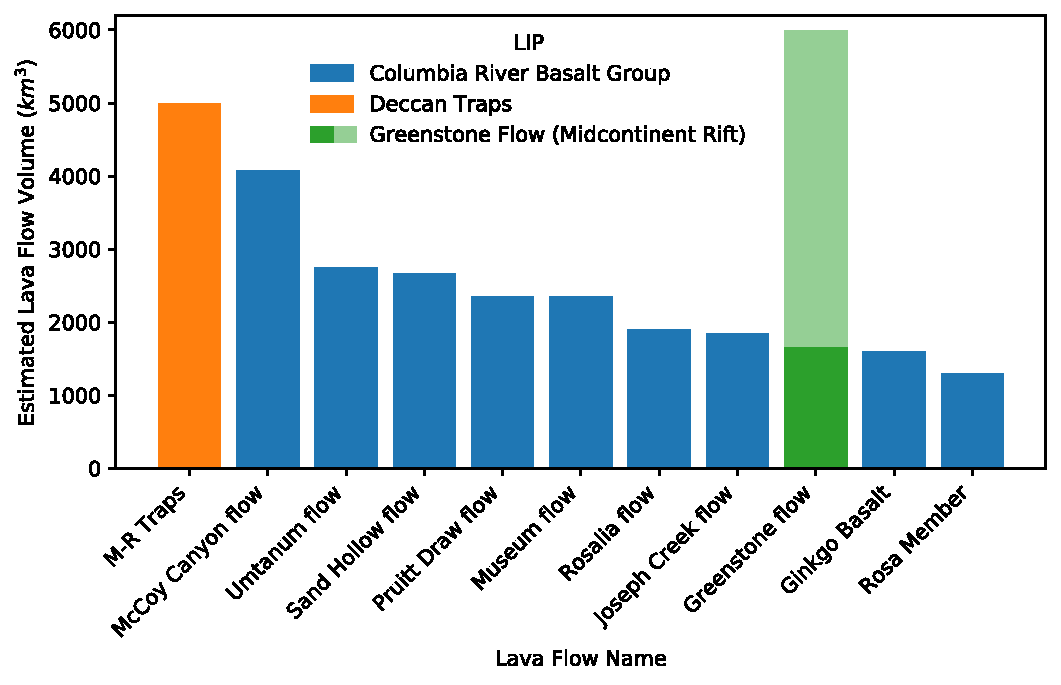
\includegraphics[width=\textwidth]{figure/Zhang2021/Lava_flow_rank.pdf}
\caption[Bar plot of ten of the world's most voluminous single mafic lava flows currently known.]{\footnotesize{Bar plot of ten of the world's most voluminous single mafic lava flows currently known. With an estimated minimum volume of $\sim$1650 km$^3$ and likely volume as high as $\sim$6000 km$^3$, the Greenstone Flow from the 1.1 Ga Midcontinent Rift stands amongst the giant lava flows from the Deccan Traps and Columbia River basalts. M-R Traps = Mahabaleshwar--Rajahmundry lava flow in the Deccan Traps. Volume estimates from \cite{Self2008a}, \cite{Bryan2010a}, \cite{Longo1984a}, and \cite{Doyle2016a}.}}
\label{fig:lava_flow_rank}
\end{figure}

One distinctive feature of the Beaver River diabase is its inclusions of anorthosite xenoliths. In the southern part of the Beaver Bay Complex, the Beaver River diabase occurs as dikes and sills, typically including anorthosites with various sizes ranging from centimeters to over 150 meters (Figs. \ref{Chap_BBC_Geologic_map}, \ref{fig:Chap_BBC_Field_photo}; \citealp{Grout1939a, Morrison1983a}). The diabase in this region intrudes the Palisade rhyolite of the North Shore Volcanic Group (Fig. \ref{Chap_BBC_Geologic_map}), which has a $^{206}$Pb/$^{238}$U date of 1093.94 $\pm$ 0.28 Ma (2$\sigma$ analytical uncertainty is presented for CA-ID-TIMS dates throughout this work; \cite{Swanson-Hysell2019a}). The Beaver River diabase is locally intruded by the Silver Bay intrusions (Fig. \ref{Chap_BBC_Geologic_map}). An aplite unit within the granophyre zone of one of these Silver Bay intrusions has a $^{206}$Pb/$^{238}$U date of 1091.61 $\pm$ 0.14 Ma \citep{Swanson-Hysell2019a}. Another arcuate, sill-like diabase body mapped as the Beaver River diabase outcrops along the eastern part of the complex (Fig. \ref{Chap_BBC_Geologic_map}; \citealp{Miller1997a}). The diabase composition there is similar to that in the south and it also contains large anorthosite xenoliths with dimensions that exceed 100 meters at Carlton Peak (Fig. \ref{Chap_BBC_Geologic_map}). The Beaver River diabase in the northern part of the complex, near the Houghtaling Creek area, typically forms narrow, near-vertical dikes instead of sheets in the southern and eastern regions (Fig. \ref{Chap_BBC_Geologic_map}; \citealp{Miller1994a}). The diabase in this region only locally contains xenoliths of anorthosite. 

Hundreds of anorthosite xenoliths have been recognized and mapped within the Beaver River diabase (Fig. \ref{Chap_BBC_Geologic_map}). Many hill tops in the Beaver Bay Complex, such as Carlton Peak and Britton Peak, are large anorthosite blocks (which lead \cite{Lawson1893a} to erroneously conclude that they were relict Archean topography). Later work established the anorthosite blocks as xenoliths, which are now extensively documented through geologic mapping of the region (Fig. \ref{Chap_BBC_Geologic_map}; \citealp{Miller2001a, Miller1988a, Miller1989a, Boerboom2004a, Boerboom2006a, Boerboom2006b, Boerboom2007a}) and outcrop-scale exposures (Fig. \ref{fig:Chap_BBC_Field_photo}). In the field, the anorthosites typically appear as subrounded to rounded, light-colored, translucent blocks that are in sharp contact with the hosting diabase (Fig. \ref{fig:Chap_BBC_Field_photo}). They also occur as exposures whose contact with the diabase is covered (Fig. \ref{fig:Chap_BBC_Field_photo}). \cite{Grout1939a} suggested that the rounded anorthosites are the result of abrasion during transportation as they were entrained by the diabase (i.e. physical weathering within a magmatic system). While the Beaver River diabase is chilled against the North Shore Volcanic Group lithologies that it intrudes, the diabase is not chilled against the margin of the anorthosite xenoliths \citep{Morrison1983a, Miller1997a}. The lack of chilled contacts is consistent with the anorthosite being at elevated temperatures and cooling at the same time as the diabase magma (Fig. \ref{fig:thermal_history_model}).

The anorthosite xenoliths are dominantly monomineralic plagioclase that has an average anorthite content of $\sim$70\% \citep{Morrison1983a, Doyle2016a}. Interstitial pyroxene and olivine are present in minor concentrations in the xenoliths. Within the Carlton Peak anorthosite xenolith, up to 10 cm oikocrysts of olivine and pyroxene can occur. Nevertheless, the overall olivine content in the anorthosites is low. Interstitial titanomagnetite-ilmenite intergrowths that exceed 100 $\mu$m can be found with microscopy and $<$20 $\mu$m Fe-Ti oxide grains can be detected with scanning electron microscopy (Fig. \ref{fig:Chap_BBC_Field_photo}). Based on textural differences \cite{Morrison1983a} divided the anorthosite xenoliths into four groups: one group which typically have well-developed granoblastic texture characterized by equigranular plagioclase crystals; another group which have interlocking, lath-shaped plagioclase crystals; an intermediate group which can have both granoblastic texture and interlocking plagioclase laths; and a brecciated group that have brittle deformation textures superposed on pre-existing textures. 

\subsection{Portage Lake Volcanics and the Greenstone Flow}

The Portage Lake Volcanics (PLV) is a $\sim$5 km thick, normally magnetized, dominantly olivine basalt to andesite volcanic succession that outcrops in northern Michigan (particularly along the Keweenaw Peninsula) as well as on Isle Royale (Fig. \ref{Chap_BBC_Geologic_map}; \citealp{Huber1973a, Cannon2001a, Green1982a}). The Greenstone Flow of the Portage Lake Volcanic Group has been recognized as one of the largest lava flows on earth (Figs. \ref{Chap_BBC_Geologic_map}, \ref{fig:lava_flow_rank}). It outcrops as the main ridge along the Keweenaw Peninsula and Isle Royale (Fig. \ref{Chap_BBC_Geologic_map}). The flow can be correlated between the two outcrop regions on the basis of geochemical, petrographic, and paleomagnetic similarity of the flow itself and the flows above and below \citep{Longo1984a}. In both outcrop regions, the Greenstone Flow is underlain by conglomerate and overlain by pyroclastic breccia \citep{Lane1911a, Huber1973a}. On the Keweenaw Peninsula, the Greenstone Flow is exposed over 90 km with a range of thickness from $\sim$100 meters to a maximum thickness of over 450 meters, dipping to the northwest (Fig. \ref{Chap_BBC_Geologic_map}; \citealp{White1960a}). On Isle Royale, the Greenstone Flow has a range of thickness from $\sim$30 meters to a maximum thickness of about 250 meters, dipping toward the southeast (Fig. \ref{Chap_BBC_Geologic_map}; \citealp{Huber1973a}). More recently, \cite{Doyle2016a} estimated that the total aerial extent of the Greenstone Flow could be up to $\sim$20000 km$^2$ by connecting it to the region of the Beaver Bay Complex. Taking thickness range of 100 to 300 meters, \cite{Doyle2016a} estimated a total volume of 2000 to 6000 km$^3$. This volume range makes the Greenstone Flow one of the largest, if not the largest, single mafic lava flows on Earth (Fig. \ref{fig:lava_flow_rank}).

According to the mineralogical and textural attributes, the Greenstone Flow can be divided into four zones from bottom to top --- a lower ophitic zone, a ``pegmatoid'' or heterolithic zone, an upper ophitic zone, and an amygdaloidal zone \citep{Cornwall1951b}. The heterolithic zone contains lenses to layers of coarse-grained granophyric gabbro that are referred to in the literature as ``pegmatoid.'' Zircon crystallized in these layers have enabled the heterolithic zone to be targeted for U-Pb geochronology \citep{Davis1990a, Swanson-Hysell2019a}. A $^{206}$Pb/$^{238}$U zircon date of 1091.59 $\pm$ 0.27 Ma for the Greenstone Flow was developed from a sample from this zone in \cite{Swanson-Hysell2019a}. The Greenstone Flow is typically interpreted to represent emplacement of a single body of magma that then underwent in situ differentiation \citep{Huber1973a, Davis1990a}. \cite{Doyle2016a} favored a distinct model in which the Greenstone Flow is a composite unit, which they interpret to be indicated by lithologic zonation of ophitic basalt forming the upper and lower zones and an interior zone composed of prismatic ferrogabbro to granophyric monzodiorite. They envision emplacement of the Greenstone Flow started with voluminous eruption of olivine tholeiitic magma, forming the ophitic zones which, while still crystallizing, further inflated due to subsequent injection of a more evolved basaltic magma to form intergranular gabbro in the heterolithic zone. They considered this progression to be more consistent with observed abrupt lithologic changes from the ophitic zone to the heterolithic zone over centimeter to meter scales, inclusion relationships between evolved and ophitic Greenstone Flow lithologies, and remnant blocks of initially crystallized ophitic basalt interlayered with evolved lithologies within the heterolithic zone which contains the pegmatoids. In both the \cite{Doyle2016a} model of multiple magma injections and the earlier models of in situ differentiation, it is the migration of the most evolved and volatile-rich melts within the interior of the flow in the final stages of flow crystallization that led to the formation of some aplite dikes and the coarsest segregations containing granophyre. Both models also invoke a single basaltic parental magma with distinction of where differentiation occurred in fractionally crystallizing an evolving magma chamber or solely within a single, very thick flow.

\section{Methods and Results}

\subsection{Zircon Geochronology and Geochemistry}

A sample of an anorthosite xenolith within the Beaver River diabase was collected for U-Pb geochronology along Hwy 61 across from the Silver Bay taconite plant (MS99033; 91.26358\textdegree W 47.28888\textdegree N; Fig. \ref{Chap_BBC_Geologic_map}). This sample comes from the same xenolith sampled for paleomagnetic study as site AX16 which has an exposed diameter of 27.5 meters (Fig. \ref{fig:Chap_BBC_Field_photo}). Thin sections were made from the geochronology sample as well as multiple paleomagnetic cores. As is shown in Fig. \ref{fig:Chap_BBC_Field_photo}F, plagioclase in this anorthosite xenolith have both equigranular crystals displaying a granoblastic texture and lath-shaped crystals displaying an interlocking texture. The occurrence of both textures is consistent with an interpretation that this anorthosite xenolith formed under elevated temperatures and experienced heating after initial crystallization. 

Zircons were separated from a kilogram of the anorthosite using common mineral separation methods (Supporting Information). The separated zircons were subhedral to anhedral crystals (z1-z4) and platy fragments (z5-z8). The subhedral to anhedral crystals are consistent with intercumulus crystallization within an adcumulate with platy fragments also being a common zircon morphology within anorthosites (e.g. sample AS3 of the Duluth Complex anorthositic series; \cite{Schmitz2003a}). Eight chemically abraded zircons were analyzed by isotope dilution-thermal ionization mass spectrometry (ID-TIMS) in the Boise State Isotope Geology Laboratory using EARTHTIME tracer solutions \citep{Condon2015a}. Both zircon morphologies yield indistinguishable dates. Using six of these single grain dates (and excluding two due to interpreted Pb-loss) results in a weighted mean $^{206}$Pb/$^{238}$U date of 1091.83 $\pm$ 0.21/0.37/1.15 Ma (analytical/ analytical+tracer/ analytical+tracer+decay uncertainty; Fig. \ref{fig:BBC_geochron}). 

\begin{figure}
\noindent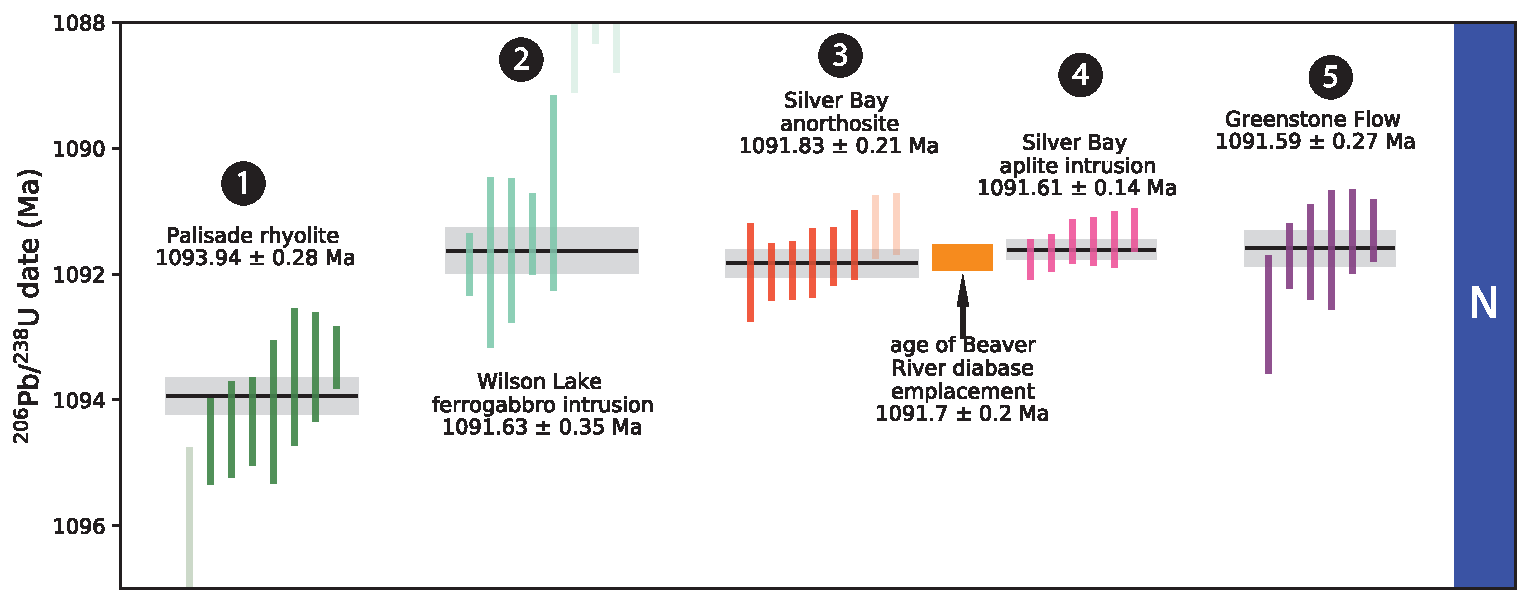
\includegraphics[width=\textwidth]{figure/Zhang2021/BBC_dates.pdf}
\caption[$^{206}$Pb/$^{238}$U zircon ages]{\footnotesize{New $^{206}$Pb/$^{238}$U zircon date of the anorthosite xenolith (dark orange) plotted in context of previously published $^{206}$Pb/$^{238}$U zircon dates from the North Shore Volcanic Group (NSVG) and other Beaver Bay Complex intrusions \citep{Swanson-Hysell2019a, Swanson-Hysell2021a}. These high-precision dates are consistent with field observations that the Beaver River diabase crosscuts the Palisade rhyolite (dark green) and is cut by the Silver Bay intrusions (pink). The estimated age of the Beaver River diabase from these constraints is shown by an orange box representing the 95$\%$ confidence interval. Each vertical bar corresponds to one $^{206}$Pb/$^{238}$U date from a single zircon crystal. The translucent bars represents zircons with interpreted Pb loss and are therefore not included in the weighted mean age calculations. Horizontal lines and gray boxes represent weighted mean $^{206}$Pb/$^{238}$U dates and their analytical uncertainty. The numbers of each geochronology sample correspond to those in Fig. \ref{Chap_BBC_Geologic_map} where locations of these samples are shown.}}
\label{fig:BBC_geochron}
\end{figure}

This date provides a tight constraint on the age of the Beaver River diabase. Previously, the maximum age constraint for the Beaver River diabase came from the relationship that it cross-cuts the Palisade rhyolite of the North Shore Volcanic Group which has a $^{206}$Pb/$^{238}$U date of 1093.94 $\pm$ 0.28 Ma  \citep{Swanson-Hysell2019a}. With this new date, we know the crystallization age of the diabase to have been near-synchronous or younger than the date from the anorthosite xenolith. The Silver Bay intrusions, from which an aplite has a $^{206}$Pb/$^{238}$U date of 1091.61 $\pm$ 0.14 Ma, \citep{Fairchild2017a}, cross-cut the Beaver River diabase. These dates constrain the diabase to have been emplaced between 1091.83 $\pm$ 0.21 and 1091.61 $\pm$ 0.14 Ma (Fig. \ref{fig:BBC_geochron}). Assuming a uniform probability of diabase emplacement between the anorthosite and aplite dates and their normal distributed uncertainties, a 95\% confidence interval on the age of the diabase can be estimated by Monte Carlo simulation. This analysis gives an age for the diabase of 1091.7 $\pm$ 0.2 Ma (95\% CI). 

\begin{figure}[h!]
\noindent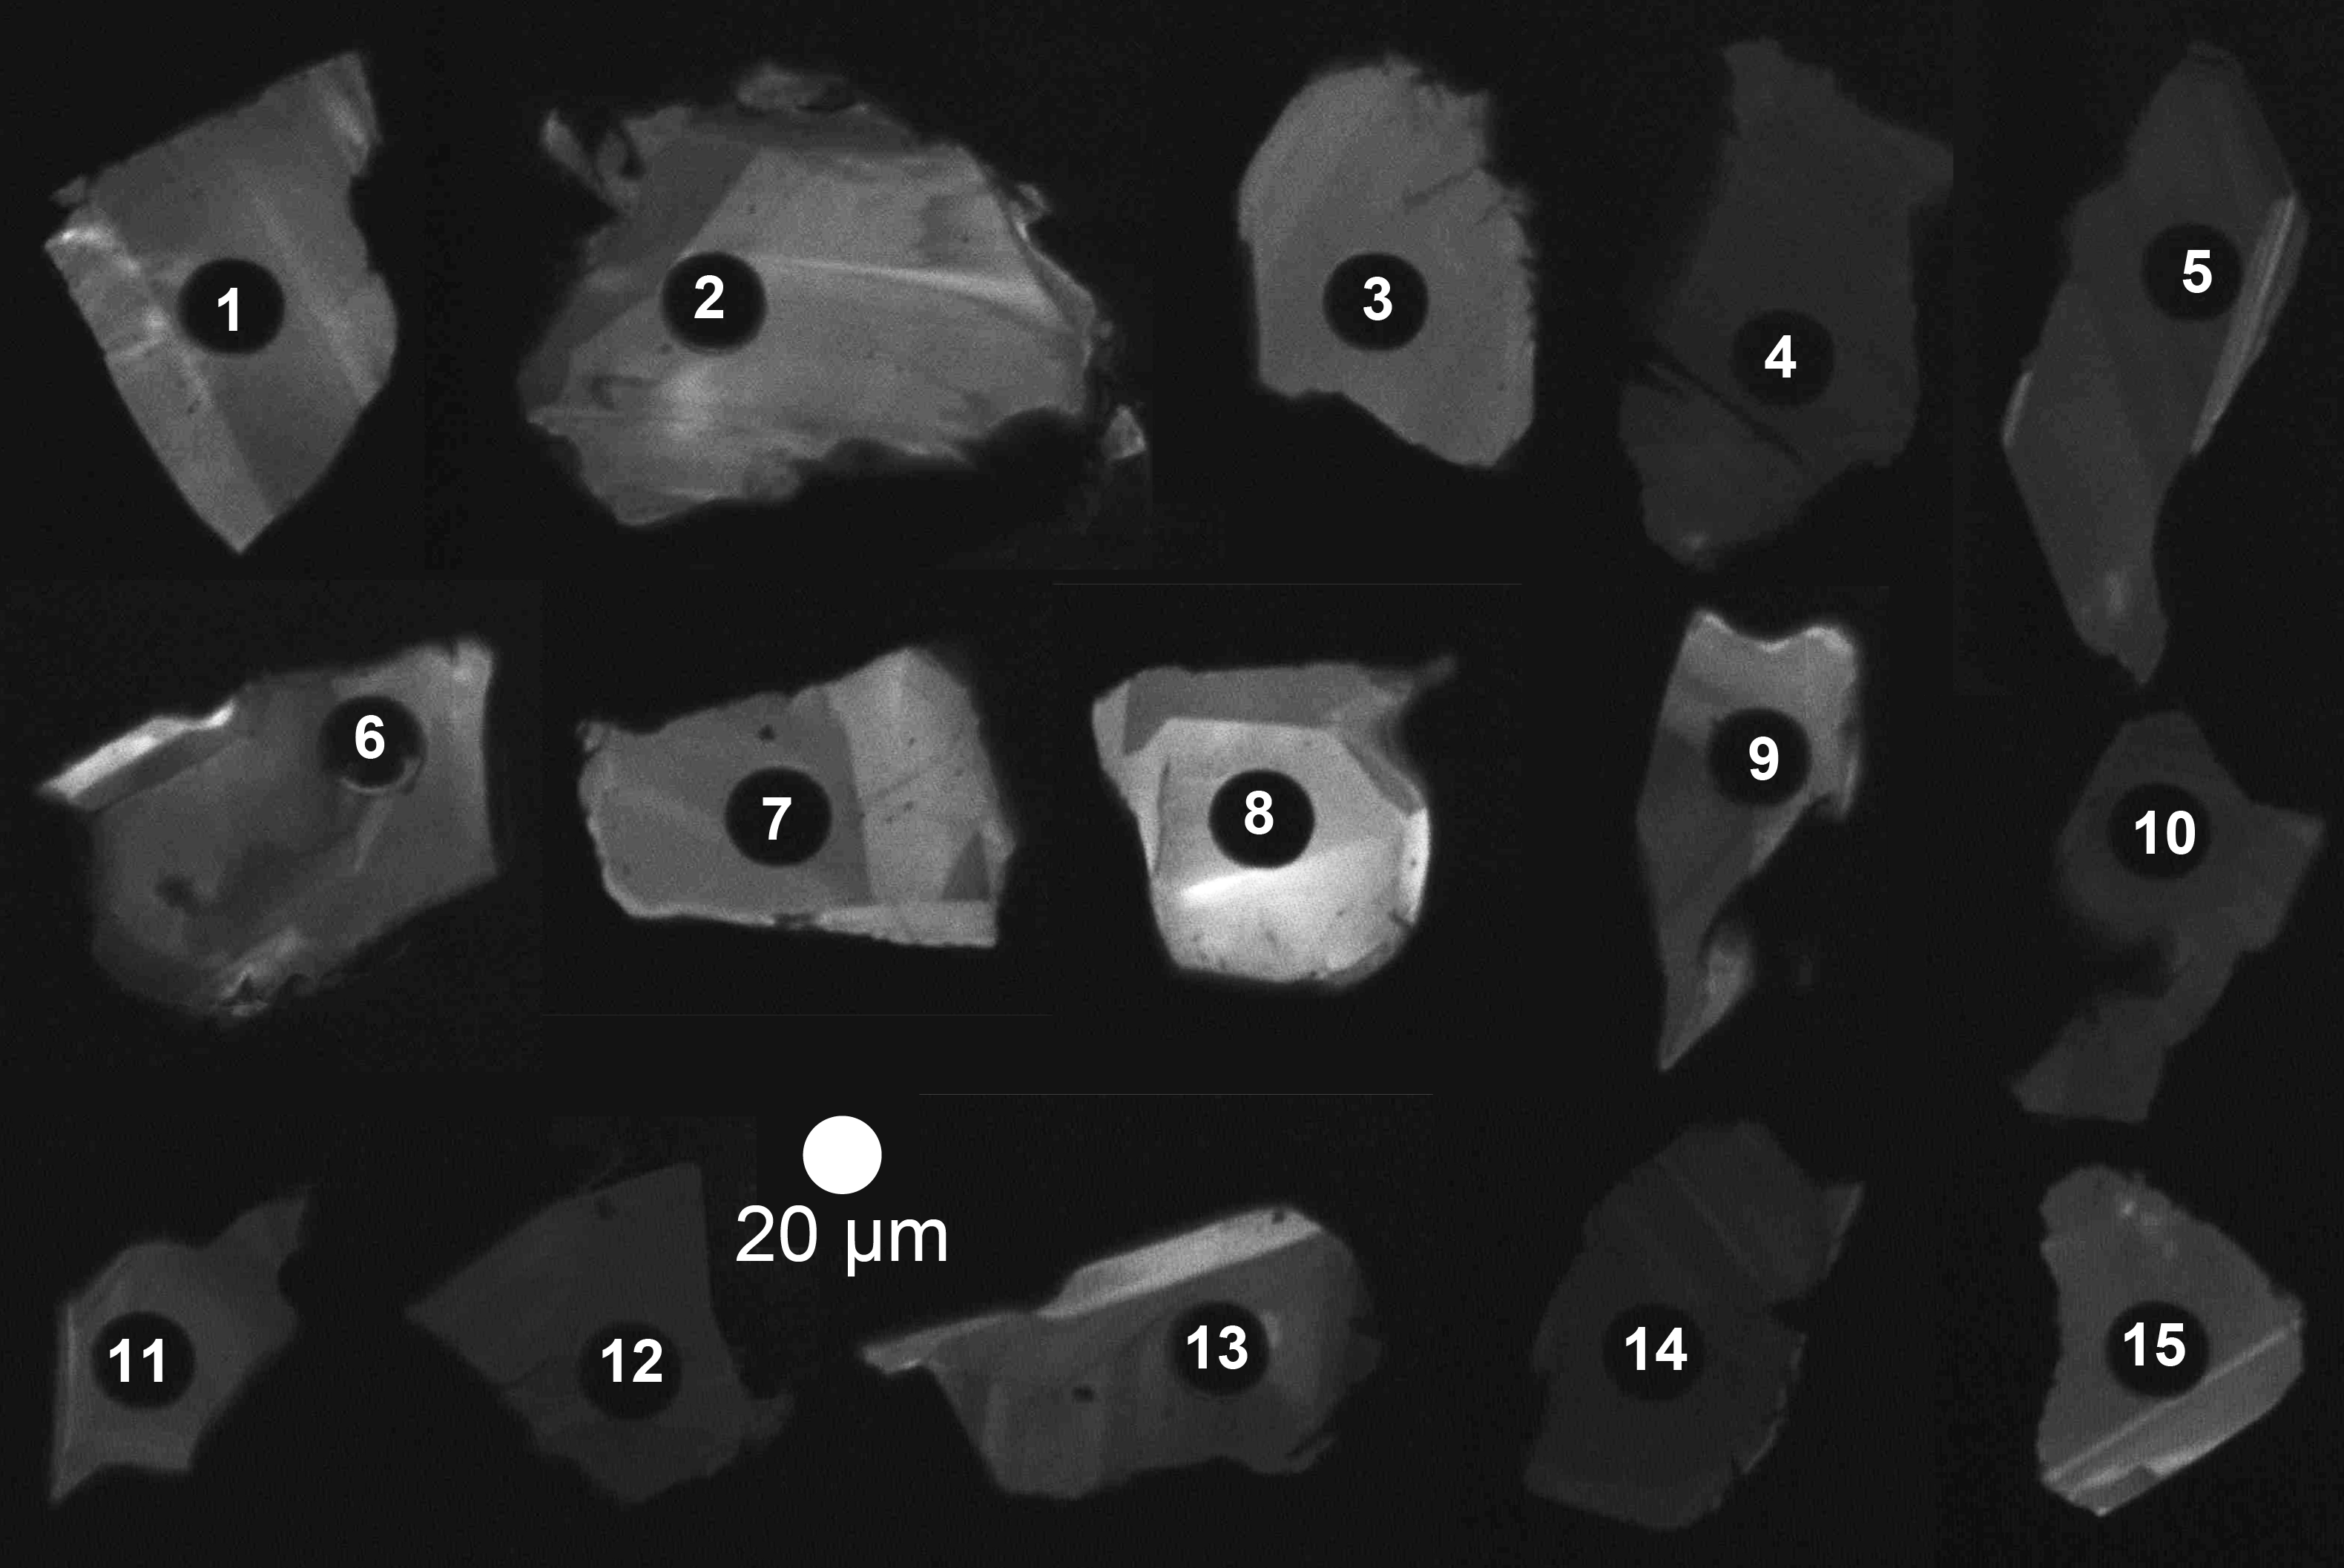
\includegraphics[width=\textwidth]{figure/Zhang2021/CL_montage.png}
\centering
\caption[Cathodoluminescnece (CL) image montage of the 15 zircons laser-ablated for trace element analysis from sample MS99033.]{\footnotesize{Cathodoluminescnece (CL) image montage of the 15 zircons laser-ablated for trace element analysis from sample MS99033. There are sharp boundaries between zones of differing CL response within many of the zircons attributable to variable REE concentrations. For example, the bright zoning in grain 15 has a thickness of $\sim$2 $\mu$m. Note that grain 1 (corresponding to spot 1) has a platy morphology, while the rest of the grains are subhedral to anhedral.}}
\label{fig:CL_image}
\end{figure}

\begin{figure}[h!]
\noindent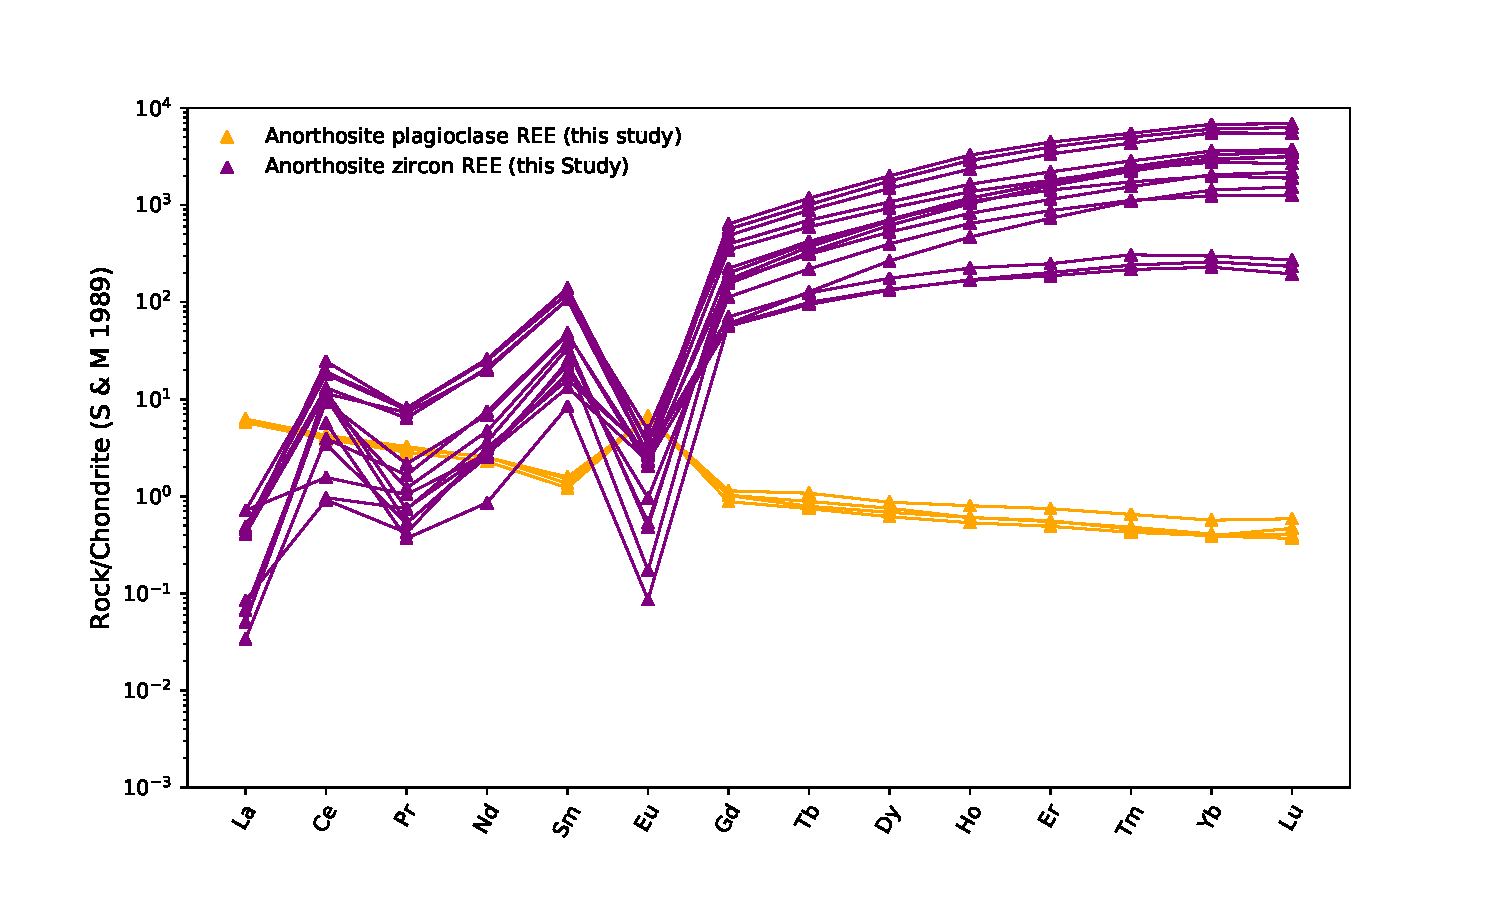
\includegraphics[width=\textwidth]{figure/Zhang2021/REE.pdf}
\centering
\caption[Rare earth element (REE) analyses for plagioclase crystals from anorthosite xenoliths and for 15 zircons from geochronology sample MS99033]{\footnotesize{Rare earth element (REE) analyses for plagioclase crystals from anorthosite xenoliths and for 15 zircons from geochronology sample MS99033 (anorthosite xenolith site AX16) developed by inductively coupled plasma mass spectrometry. All data are chrondrite-normalized \citep{Sun1989a}.}}
\label{fig:REE}
\end{figure}

An additional 15 zircons were characterized using cathodoluminescence (CL) imaging and laser ablation-inductively coupled plasma mass spectrometry (LA-ICPMS), with methods and instrumentation described in the Supporting Information. CL images reveal internal planar zones of variable brightness, often with darker interior zones and brighter outer zones (Fig. \ref{fig:CL_image}). All crystals exhibit sharp, micron-scale transitions between zones, and LA-ICPMS analyses quantify CL brightness as correlated with rare earth elements (REE) content. REE patterns in zircons exhibit a significant chondrite-normalized negative Eu anomaly (Fig. \ref{fig:REE}). The Ti-in-zircon thermometer gives a range of estimated zircon crystallization temperatures from 998\textdegree C to 860\textdegree C with a mean of $\sim$950\textdegree C (\citealp{Ferry2007a}; Supporting Information). Decreasing temperatures are correlated with deepening of the negative Eu anomaly and increasing incompatible trace element (e.g. Hf, Th) incorporation into zircon. These data are consistent with a model of magmatic zircon crystallizing from cooling and fractionating interstitial residual melt within the cumulate plagioclase framework.

\subsection{Paleomagnetism}

We collected paleomagnetic cores that are 2.5 cm in diameter along the southern and eastern Beaver Bay Complex with a particular focus on acquiring paired sites of anorthosite xenoliths and their local diabase hosts. Sample cores were collected using a hand-held gasoline-powered drill and were oriented using a magnetic compass as well as a sun compass when possible. Sun compass orientations were preferentially used for determining the sample azimuth. Typically, 7-10 cores were collected for each anorthosite xenolith and their diabase hosts. A total of 17 diabase and 22 anorthosite sites were sampled (Table \ref{tab:Pmag_site_data}). A table that summarizes the measured dimensions of each anorthosite xenolith sampled and the distance between each anorthosite paleomagnetic site and closest diabase host site is provided in the Supporting Information.  

Samples underwent step-wise demagnetization and analyses in the magnetically-shielded room at the UC Berkeley Paleomagnetism Lab. 7 sites from the Beaver River diabase underwent alternating field (AF) demagnetization with peak fields from 1 mT to 130 mT. An ASC TD-48SC thermal demagnetizer was used to demagnetize 10 diabase sites and all 22 anorthosite sites in a step-wise manner, with reduced step increments between 540\textdegree C and 585\textdegree C. The typical magnetic field inside the shielded room is $<$500 nT and the field inside the thermal demagnetizer chamber is $<$10 nT. The quartz glass sample rod of the UC Berkeley system is typically measured at 5 $\times$ 10$^{-12}$ Am$^{2}$. All remanence measurements were made on a 2G Enterprises DC-SQUID superconducting rock magnetometer equipped with inline AF coils and an automated sample changer system. The PmagPy software package was used to implement least-square fits to specimen demagnetization data \citep{Tauxe2016a}. Measurement level data are available within the MagIC database (\url{https://earthref.org/MagIC/doi/10.1029/2021GC009909})

\begin{figure}
\centering 
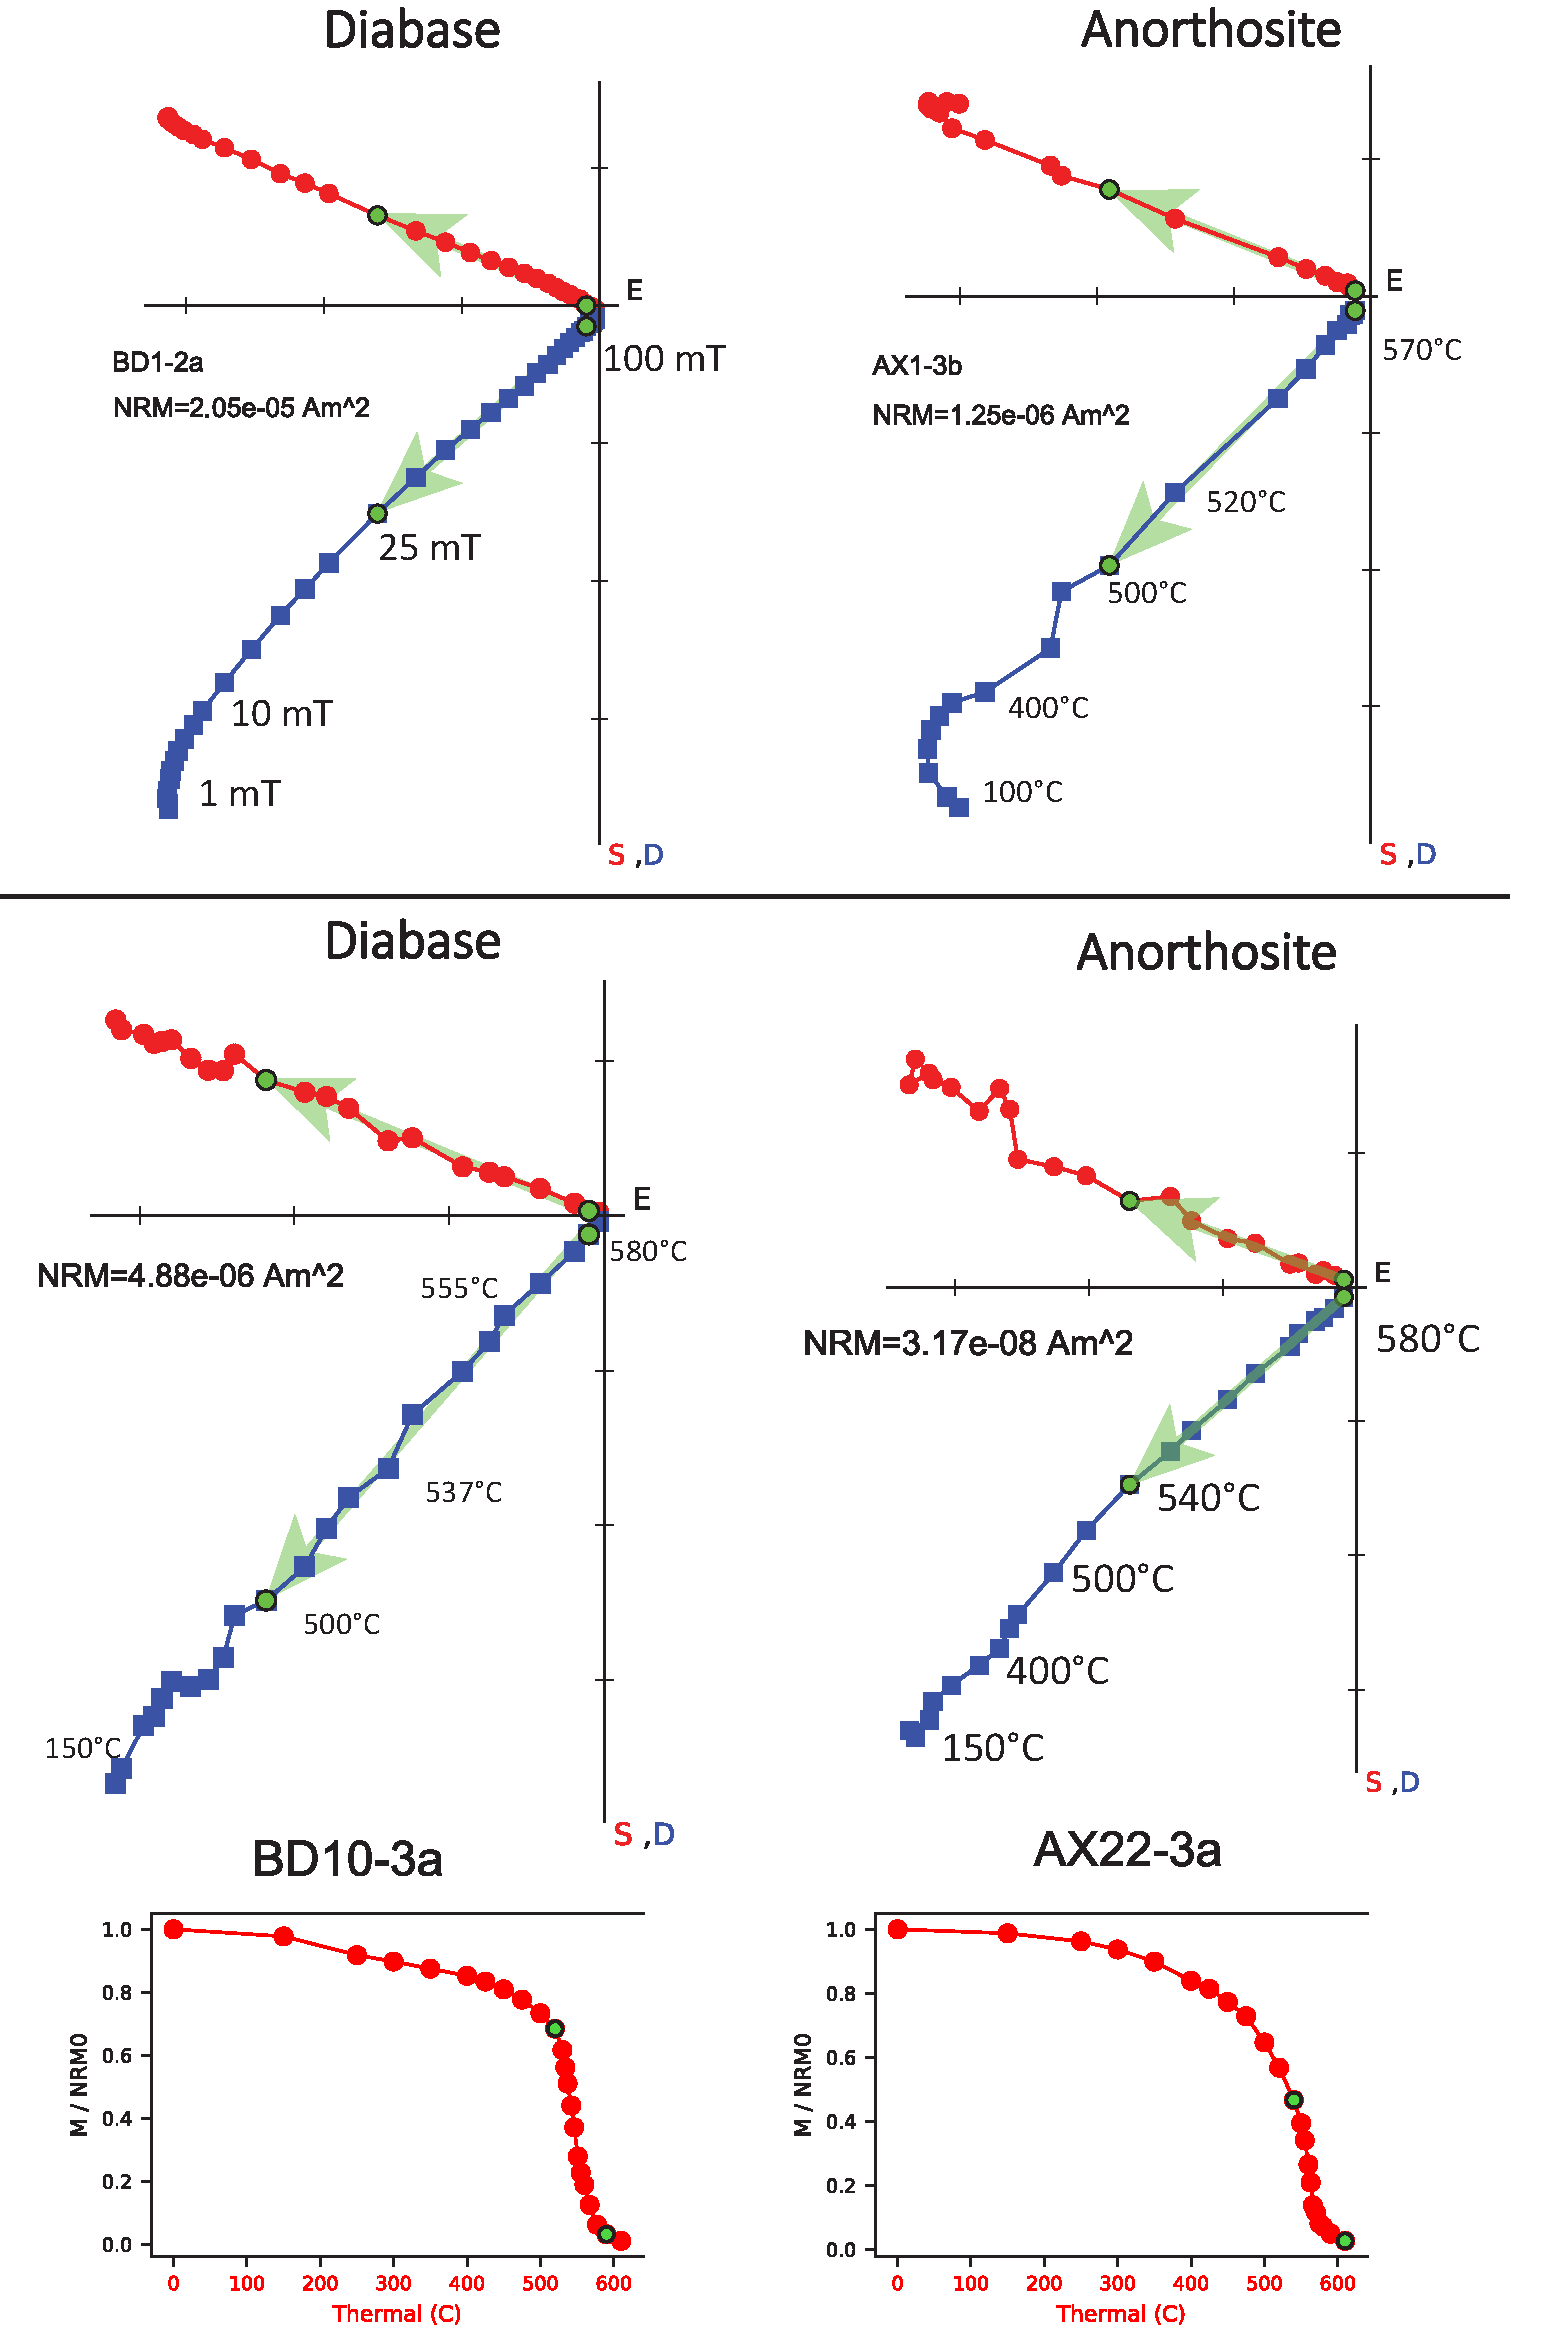
\includegraphics[width=0.65\textwidth]{figure/Zhang2021/Demag.pdf}
\caption[Example orthogonal vector demagnetization diagrams for diabase and anorthosite specimens]{\small{Example orthogonal vector demagnetization diagrams for diabase and anorthosite specimens. Anorthosite site AX1 is a xenolith within the diabase sampled as BD1. Similarly, AX22 is from a xenolith within the BD10 diabase. Both AF and thermal demagnetization show dominantly univectoral decay of characteristic remanent magnetizations (ChRM) toward the origin after removal of minimal secondary components. The data show very similar ChRM directions between the paired diabase and anorthosite xenoliths sites. Representative magnetization intensity versus thermal demagnetization step plots are paired with orthogonal vector plots for specimen BD10-3a and AX22-3a.}}
\label{fig:Demag}
\end{figure}

For both the diabase and anorthosite demagnetization, principal component analyses show that an origin trending characteristic remanent magnetization (ChRM) can be isolated after the removal of a minimal secondary component during the first few low coercivity ($<$10 mT) or low temperature ($<$200\textdegree C) demagnetization steps (Fig. \ref{fig:Demag}). The ChRMs typically unblock through thermal demagnetization steps from $\sim$500\textdegree C to $\sim$580\textdegree C, consistent with the component being held by low-titanium titanomagnetite. We interpret this component as a primary remanent magnetization acquired during the emplacement and cooling of the Beaver River diabase.

The site mean paleomagnetic directions are shown in Table \ref{tab:Pmag_site_data}. We present both AF and thermal demagnetization results for the Beaver River diabase as both methods are effective in removing the secondary components and isolating the coherent and univectoral ChRM. Based on specimen and site level demagnetization behavior and the proximity between paired paleomagnetic sites of the anorthosite xenoliths and the diabase, we grouped the anorthosite xenoliths and their diabase hosts into individual cooling units and calculated a paleomagnetic pole position from the mean of the cooling unit virtual geomagnetic poles (Fig. \ref{fig:Direction_pairs}). 

\begin{figure}
\noindent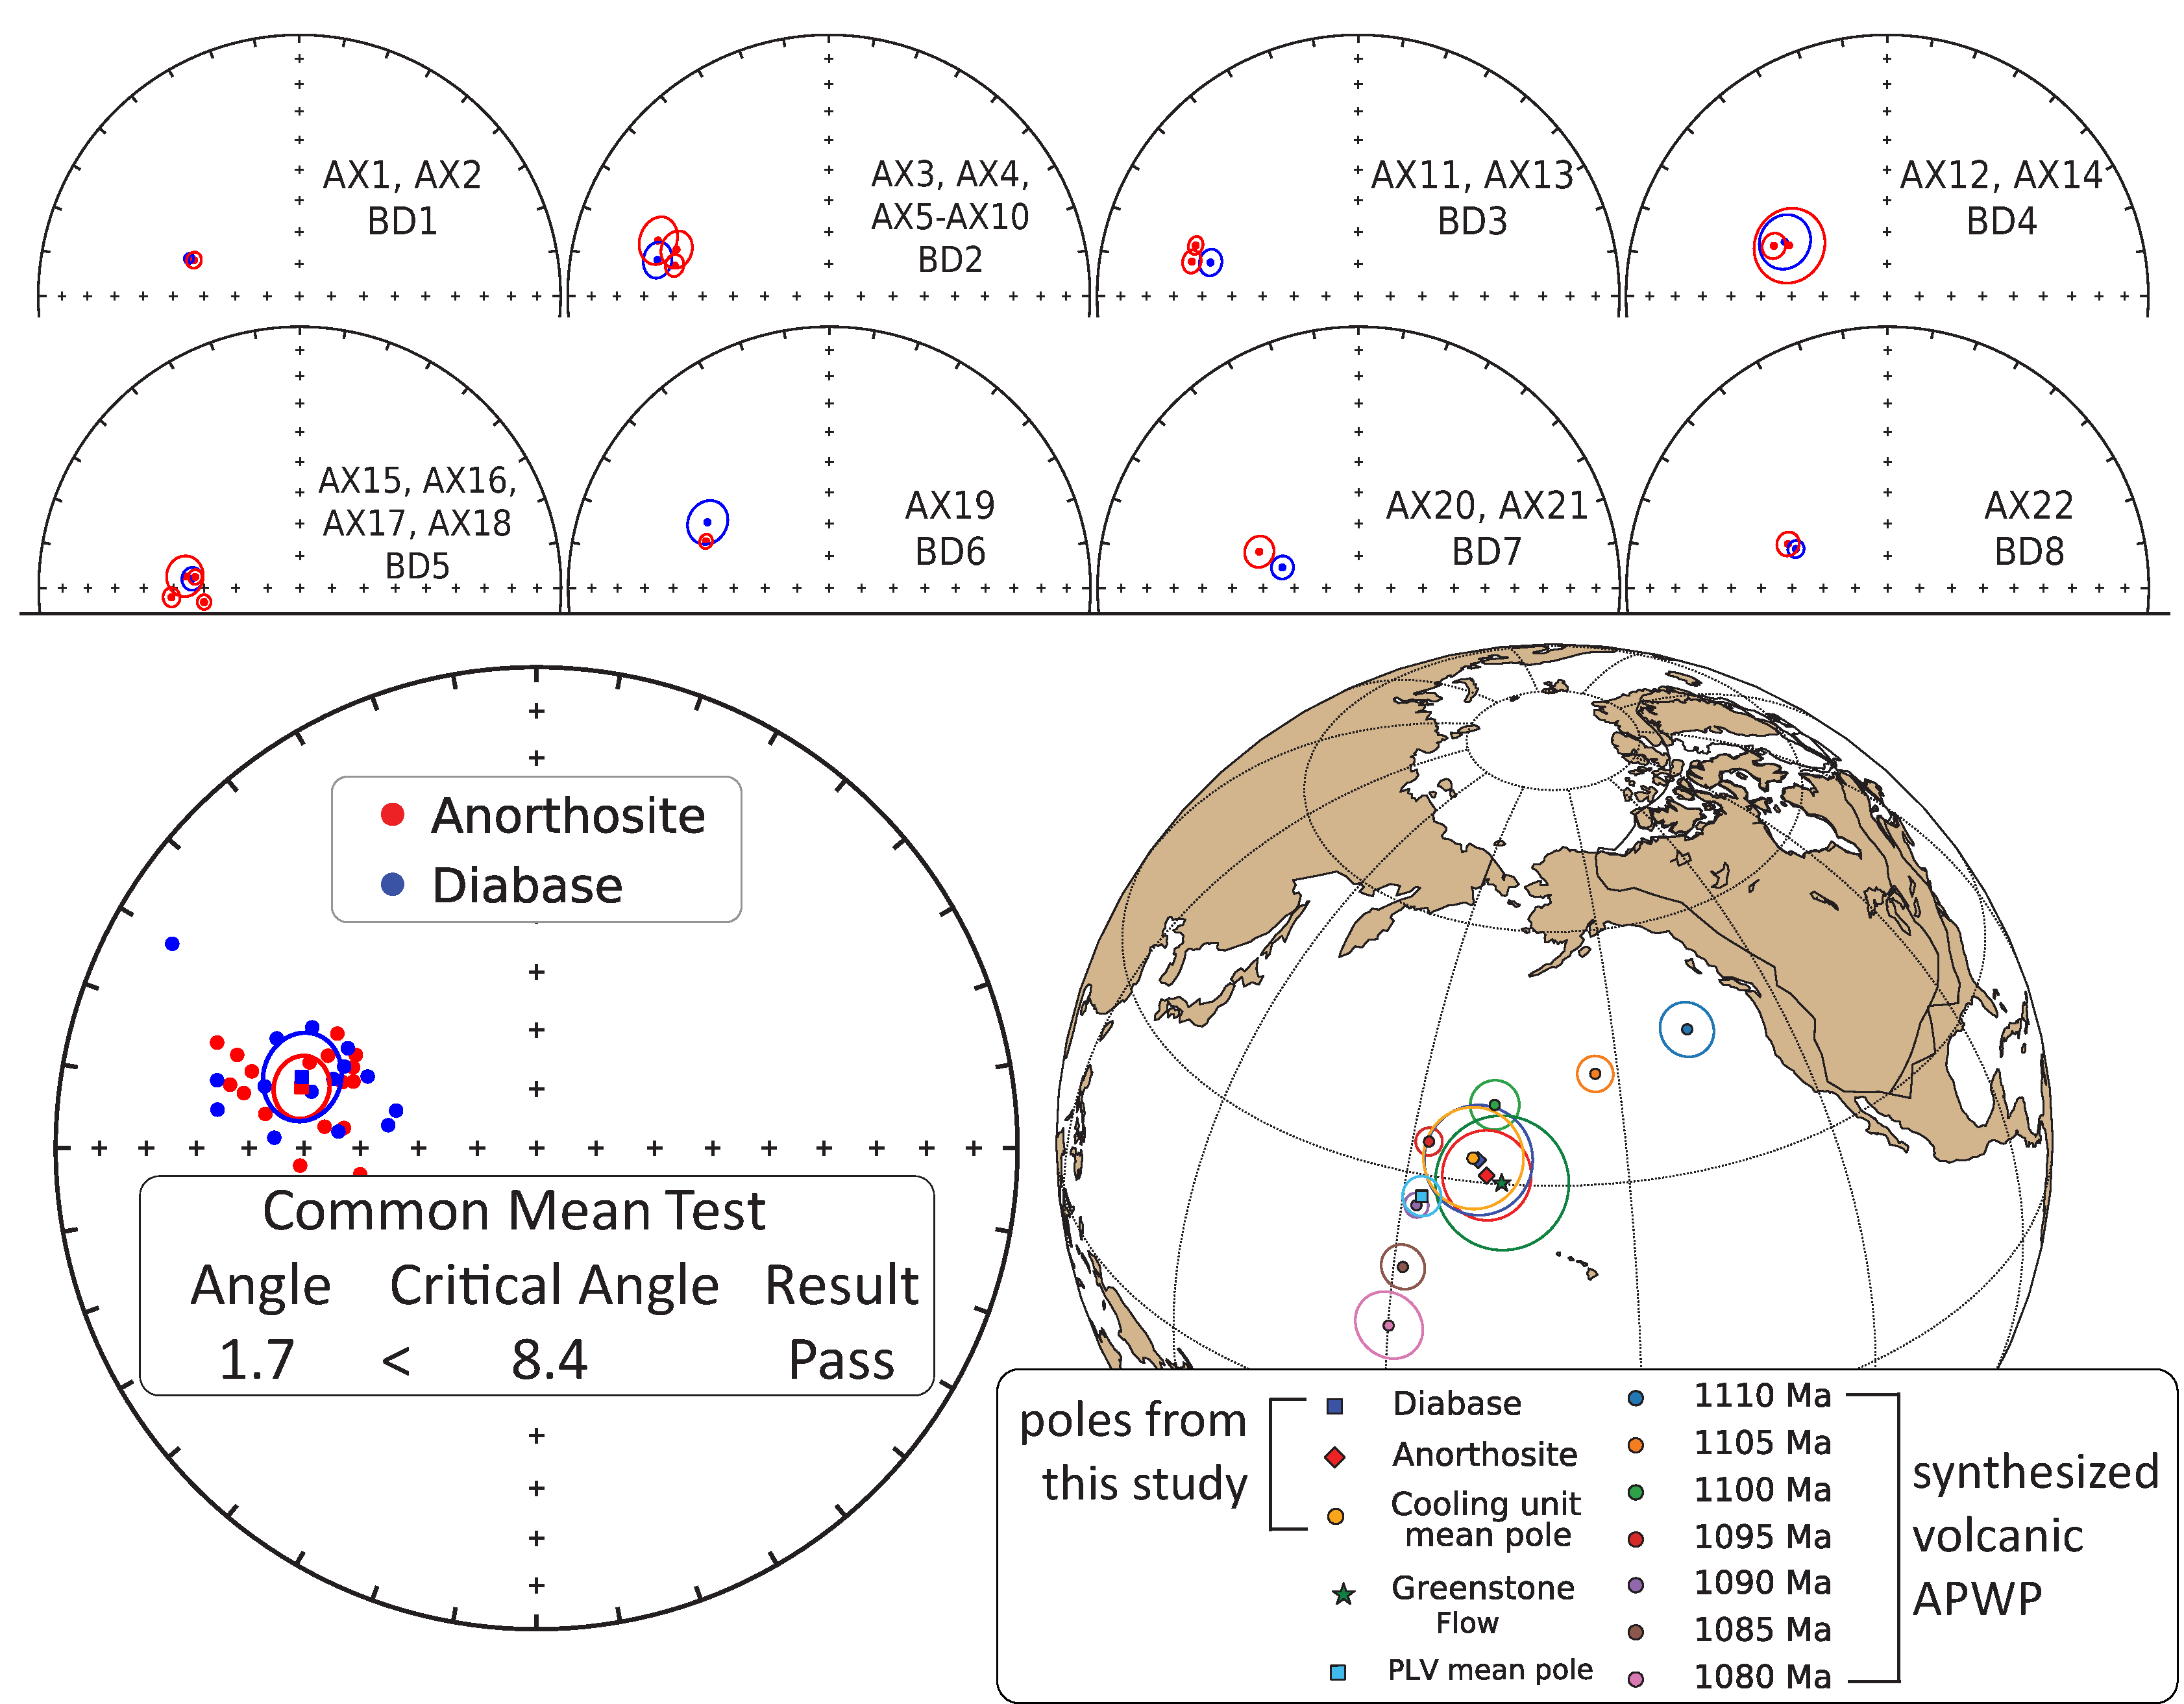
\includegraphics[width=\textwidth]{figure/Zhang2021/Direction_pairs.pdf}
\caption[Summary equal area plots and paleomagnetic pole plots]{\small{Top: Equal area plots of paleomagnetic directions from the anorthosite xenoliths and their local diabase hosts. AX: anorthosite xenolith site; BD: Beaver River diabase site. Bottom: Site mean paleomagnetic directions from the Beaver River diabase and anorthosite xenoliths are plotted on equal area plots. The anorthosite and diabase sites share a common mean as summarized by the results of the \cite{McFadden1990a} common mean test. Mean paleomagnetic pole positions of all diabase sites, all anorthosite sites, as well as a grand mean pole developed by grouping the anorthosite and diabase sites into individual cooling units are plotted against a synthesized Laurentia APWP based on poles from Midcontinent Rift volcanics and sedimentary rocks \citep{Swanson-Hysell2019a}. The paleomagnetic poles from the diabase and anorthosite are indistinguishable with the Greenstone Flow pole developed by \cite{Foucher2018a}, but they all are distinct from the Portage Lake Volcanics mean pole \citep{Swanson-Hysell2019a}. All directions shown are tilt corrected.}}
\label{fig:Direction_pairs}
\end{figure}

Tilt-correcting the paleomagnetic directions to paleohorizontal is necessary for developing accurate paleomagnetic poles from the diabase and the anorthosite xenoliths to be compared to the Keweenawan Track apparent polar wander path (APWP; Fig. \ref{fig:Direction_pairs}; \citealp{Swanson-Hysell2019a}). For intrusive igneous rocks, tilt corrections can be difficult to constrain due to the lack of a clear paleohorizontal reference. Many paleomagnetic studies of Midcontinent Rift intrusive rocks in the Lake Superior region did not apply tilt corrections to their data \cite[e.g.][]{Beck1969a, Beck1970a, Books1966a}. However, we can determine the structural orientation of the Beaver River diabase using the abundant igneous fabric orientations measured on the diabase as well as bedding orientations measured from adjacent volcanic units \citep{Boerboom2004a, Boerboom2006a, Boerboom2006b, Boerboom2007a, Miller2001a}. We compile the igneous layering measurements from the Beaver River diabase and the volcanic bedding orientations from the Schroeder-Lutsen basalt which is overlying the Beaver Bay Complex (Fig. \ref{Chap_BBC_Geologic_map}). Despite the uncertainties associated with using igneous fabrics orientations as paleohorizontal references, the mean tilt orientations of the fabrics of the Beaver River diabase and the volcanic bedding orientations of the Schroeder-Lutsen basalt are similar (diabase overall dip direction - dip: 128.5 - 10.2; basalt dip direction - dip: 142.2 - 13.6). We combine the structural measurements from the Beaver River diabase and the Schroeder-Lutsen basalt and derived two sets of tilt corrections for the paleomagnetic directions of the diabase and anorthosite (dip direction - dip in the southern Beaver Bay complex: 128.7 - 12.9; in the eastern Beaver Bay Complex: 145.6-13.1, Supporting Information). The advantage of using the structural orientations from the Schroeder-Lutsen basalt is that the arcuate shape of the Beaver River diabase intrusions is nicely captured by the variation of lava dip directions while the dip angles of the basalt and diabase are very similar (Fig. \ref{Chap_BBC_Geologic_map}).

The tilt-corrected ChRMs in both lithologies are west-northwest and down, yielding good specimen-level and site-level consistency (Figs. \ref{fig:Demag} and \ref{fig:Direction_pairs}). Close directional similarities between each anorthosite xenolith and their host diabase are supported by 9 out of a total of 17 diabase-anorthosite paleomagnetic site pairs passing a common mean test \citep{McFadden1990a}. The overall mean directions between the two lithologies are indistinguishable as they also pass a common mean test (Fig. \ref{fig:Direction_pairs}, \citealp{McFadden1990a}). For the anorthosite sites that do not pass a common mean test with their diabase hosts, they nevertheless have coherent specimen-level directions that are close to their host diabase directions (Fig. \ref{fig:Direction_pairs}). We also plot the tilt-corrected mean pole of sites from both lithologies (diabase: 32.5\textdegree N, 189.5\textdegree E, N = 15, A95 = 6.3, k = 37.4; anorthosite: 30.9\textdegree N, 190.8\textdegree E, N = 17, A95: 5.2, k = 48.5; Table. \ref{tab:Pmag_site_data}) in context of a previously synthesized APWP from the volcanics of the Midcontinent Rift \citep{Swanson-Hysell2019a} and show the poles to lie near the expected 1090 Ma and 1095 Ma pole positions (Fig. \ref{fig:Direction_pairs}). The mean pole position of the interpreted cooling units (32.7\textdegree N, 188.8\textdegree E, N = 15, A95 = 5.9, k = 41) lies close to the mean pole position derived from the ca. 1092 Ma Portage Lake Volcanics (Fig. \ref{fig:Direction_pairs}), consistent with the coeval magmatic activity between the Beaver River diabase and the Portage Lake Volcanics. If it is included in future Laurentia APWP compilations, it is this cooling unit mean pole paired with the estimated diabase emplacement age of 1091.7 $\pm$ 0.2 Ma that should be used.


\begin{sidewaystable}
\scriptsize
\caption[Summary of new site level paleomagnetic data for the Beaver River diabase and anorthosite xenoliths.]{\footnotesize Summary of new site level paleomagnetic data for the Beaver River diabase and anorthosite xenoliths. n/N: number of samples/sites analyzed and included in the site/grand mean; $dec_{is}$ \& $inc_{is}$: in situ mean declination and inclination for the site; $dec_{tc}$ \& $inc_{tc}$: tilt-corrected mean declination and inclination for the site; k: Fisher precision parameter; R: resultant vector length; $\alpha$95: 95\% confidence limit in degrees; VGP lat—latitude of the virtual geomagnetic pole for the site; VGP lon—longitude of the virtual geomagnetic pole for the site. Full measurement level data are available within the MagIC database. \url{https://earthref.org/MagIC/doi/10.1029/2021GC009909}.}
\centering
\begin{tabular}{cccccccccccccc}
\hline
site             & lat  & lon   & n/N  & $dec_{is}$ & $inc_{is}$ & $dec_{tc}$ & $inc_{tc}$ & k     & $\alpha_{95}$ & VGP $lat_{is}$ & VGP $lon_{is}$ & VGP $lat_{tc}$ & VGP $lon_{tc}$ \\
\hline
AX1              & 47.2 & -91.4 & 8.0  & 293.3   & 42.6         & 288.8   & 54.9    & 536.0 & 2.4                     & 33.4        & 180.0       & 37.1         & 193.2        \\
AX2              & 47.2 & -91.4 & 9.0  & 282.0   & 31.3         & 277.2   & 42.6    & 145.0 & 4.3                     & 20.4        & 181.8       & 22.6         & 191.1        \\
AX3              & 47.6 & -90.9 & 10.0 & 290.4   & 28.2         & 285.1   & 38.6    & 69.0  & 5.9                     & 24.7        & 174.5       & 25.9         & 183.7        \\
AX4              & 47.6 & -90.9 & 7.0  & 291.9   & 20.0         & 288.3   & 30.7    & 91.0  & 6.4                     & 22.3        & 169.8       & 24.4         & 177.2        \\
AX5-10           & 47.6 & -90.9 & 14.0 & 286.2   & 29.1         & 280.7   & 38.1    & 269.5 & 2.5                     & 22.3        & 178.1       & 22.7         & 186.5        \\
AX11             & 47.4 & -91.2 & 8.0  & 284.9   & 23.5         & 281.7   & 35.2    & 305.0 & 3.2                     & 19.1        & 176.3       & 22.0         & 184.1        \\
AX12             & 47.3 & -91.3 & 6.0  & 299.9   & 42.5         & 297.3   & 55.2    & 36.0  & 11.3                    & 37.8        & 175.1       & 43.0         & 188.4        \\
AX13             & 47.4 & -91.2 & 9.0  & 289.8   & 23.0         & 287.3   & 35.1    & 434.0 & 2.5                     & 22.2        & 172.4       & 25.7         & 180.0        \\
AX14             & 47.3 & -91.3 & 7.0  & 296.9   & 38.2         & 293.9   & 50.8    & 256.0 & 3.8                     & 33.7        & 174.5       & 38.2         & 186.1        \\
AX15             & 47.3 & -91.3 & 8.0  & 282.9   & 42.3         & 275.8   & 53.5    & 86.0  & 6.0                     & 26.2        & 187.2       & 27.9         & 199.8        \\
AX16             & 47.3 & -91.3 & 8.0  & 273.7   & 39.1         & 265.8   & 49.2    & 396.0 & 2.8                     & 18.5        & 191.6       & 19.0         & 202.9        \\
AX17             & 47.3 & -91.3 & 8.0  & 273.6   & 49.8         & 261.6   & 59.6    & 647.0 & 2.2                     & 24.3        & 198.3       & 23.7         & 213.5        \\
AX18             & 47.3 & -91.3 & 9.0  & 283.8   & 45.5         & 276.0   & 56.9    & 535.0 & 2.2                     & 28.5        & 188.7       & 30.2         & 202.8        \\
AX19             & 47.3 & -91.3 & 8.0  & 293.9   & 35.8         & 290.7   & 48.2    & 695.0 & 2.1                     & 30.5        & 175.4       & 34.6         & 186.0        \\
AX20             & 47.3 & -91.3 & 5.0  & 294.5   & 44.3         & 290.0   & 56.7    & 271.0 & 4.7                     & 35.1        & 180.4       & 39.0         & 194.5        \\
AX21             & 47.3 & -91.3 & 8.0  & 301.7   & 37.7         & 299.9   & 50.5    & 803.0 & 2.0                     & 36.7        & 170.4       & 42.1         & 181.7        \\
AX22             & 47.4 & -91.2 & 9.0  & 297.2   & 43.1         & 293.8   & 55.7    & 208.0 & 3.6                     & 36.3        & 177.6       & 41.0         & 191.1        \\
\hline
Anorthosite mean &      &       & 17.0 & 289.3   & 36.5         & 284.5   & 48.2    & 55.0  & 4.9                     & 28.0        & 179.6       & 30.9         & 190.8        \\
\hline
BD1              & 47.2 & -91.4 & 15.0 & 293.1   & 40.9         & 288.8   & 53.2    & 623.0 & 1.5                     & 32.4        & 179.0       & 36.1         & 191.6        \\
BD2              & 47.6 & -90.9 & 8.0  & 286.6   & 22.7         & 282.0   & 32.6    & 122.0 & 5.0                     & 19.9        & 175.0       & 21.0         & 182.8        \\
BD3              & 47.4 & -91.2 & 8.0  & 286.6   & 29.8         & 282.8   & 41.6    & 212.0 & 3.8                     & 22.9        & 177.9       & 25.8         & 186.9        \\
BD4              & 47.3 & -91.3 & 8.0  & 300.2   & 40.7         & 297.9   & 53.4    & 47.0  & 8.2                     & 37.1        & 173.6       & 42.3         & 186.0        \\
BD5              & 47.3 & -91.3 & 8.0  & 282.7   & 44.8         & 274.8   & 56.0    & 271.0 & 3.4                     & 27.4        & 188.9       & 28.9         & 202.6        \\
BD6              & 47.3 & -91.3 & 9.0  & 300.0   & 33.2         & 298.3   & 46.0    & 64.0  & 6.5                     & 33.4        & 169.2       & 38.6         & 178.9        \\
BD7              & 47.3 & -91.3 & 7.0  & 292.4   & 53.1         & 285.0   & 65.3    & 305.0 & 3.5                     & 38.5        & 189.2       & 41.3         & 208.3        \\
BD8              & 47.2 & -91.4 & 10.0 & 287.9   & 52.8         & 278.8   & 64.5    & 300.0 & 2.8                     & 35.3        & 191.8       & 37.1         & 209.9        \\
BD9              & 47.2 & -91.3 & 7.0  & 278.2   & 33.8         & 272.3   & 44.6    & 55.0  & 8.2                     & 19.0        & 185.7       & 20.4         & 195.6        \\
BD10             & 47.4 & -91.2 & 10.0 & 297.0   & 46.2         & 293.0   & 58.7    & 341.0 & 2.6                     & 37.8        & 180.0       & 42.2         & 195.1        \\
BD11             & 47.4 & -91.3 & 8.0  & 296.4   & 41.7         & 293.0   & 54.2    & 429.0 & 2.7                     & 35.1        & 177.1       & 39.5         & 189.9        \\
BD12             & 47.3 & -91.3 & 8.0  & 288.8   & 38.1         & 284.1   & 50.1    & 141.0 & 4.7                     & 28.1        & 180.4       & 31.3         & 191.8        \\
BD13             & 47.5 & -91.1 & 8.0  & 280.4   & 22.4         & 276.9   & 33.6    & 341.0 & 3.0                     & 15.6        & 179.2       & 18.0         & 186.7        \\
BD15             & 47.7 & -90.6 & 8.0  & 300.1   & 2.3          & 299.3   & 14.2    & 119.0 & 5.1                     & 20.6        & 156.9       & 24.8         & 161.7        \\
BD17             & 47.4 & -91.2 & 8.0  & 295.1   & 28.5         & 292.9   & 41.0    & 550.0 & 2.4                     & 28.0        & 170.8       & 32.3         & 179.3        \\
\hline
Diabase mean     &      &       & 15.0 & 291.0   & 35.7         & 286.9   & 47.7    & 51.6  & 5.0                     & 29.0        & 178.2       & 32.5         & 189.5       \\
\hline
\end{tabular}
\label{tab:Pmag_site_data}
\end{sidewaystable}


\subsection{Thermal history model}

\begin{figure}
\noindent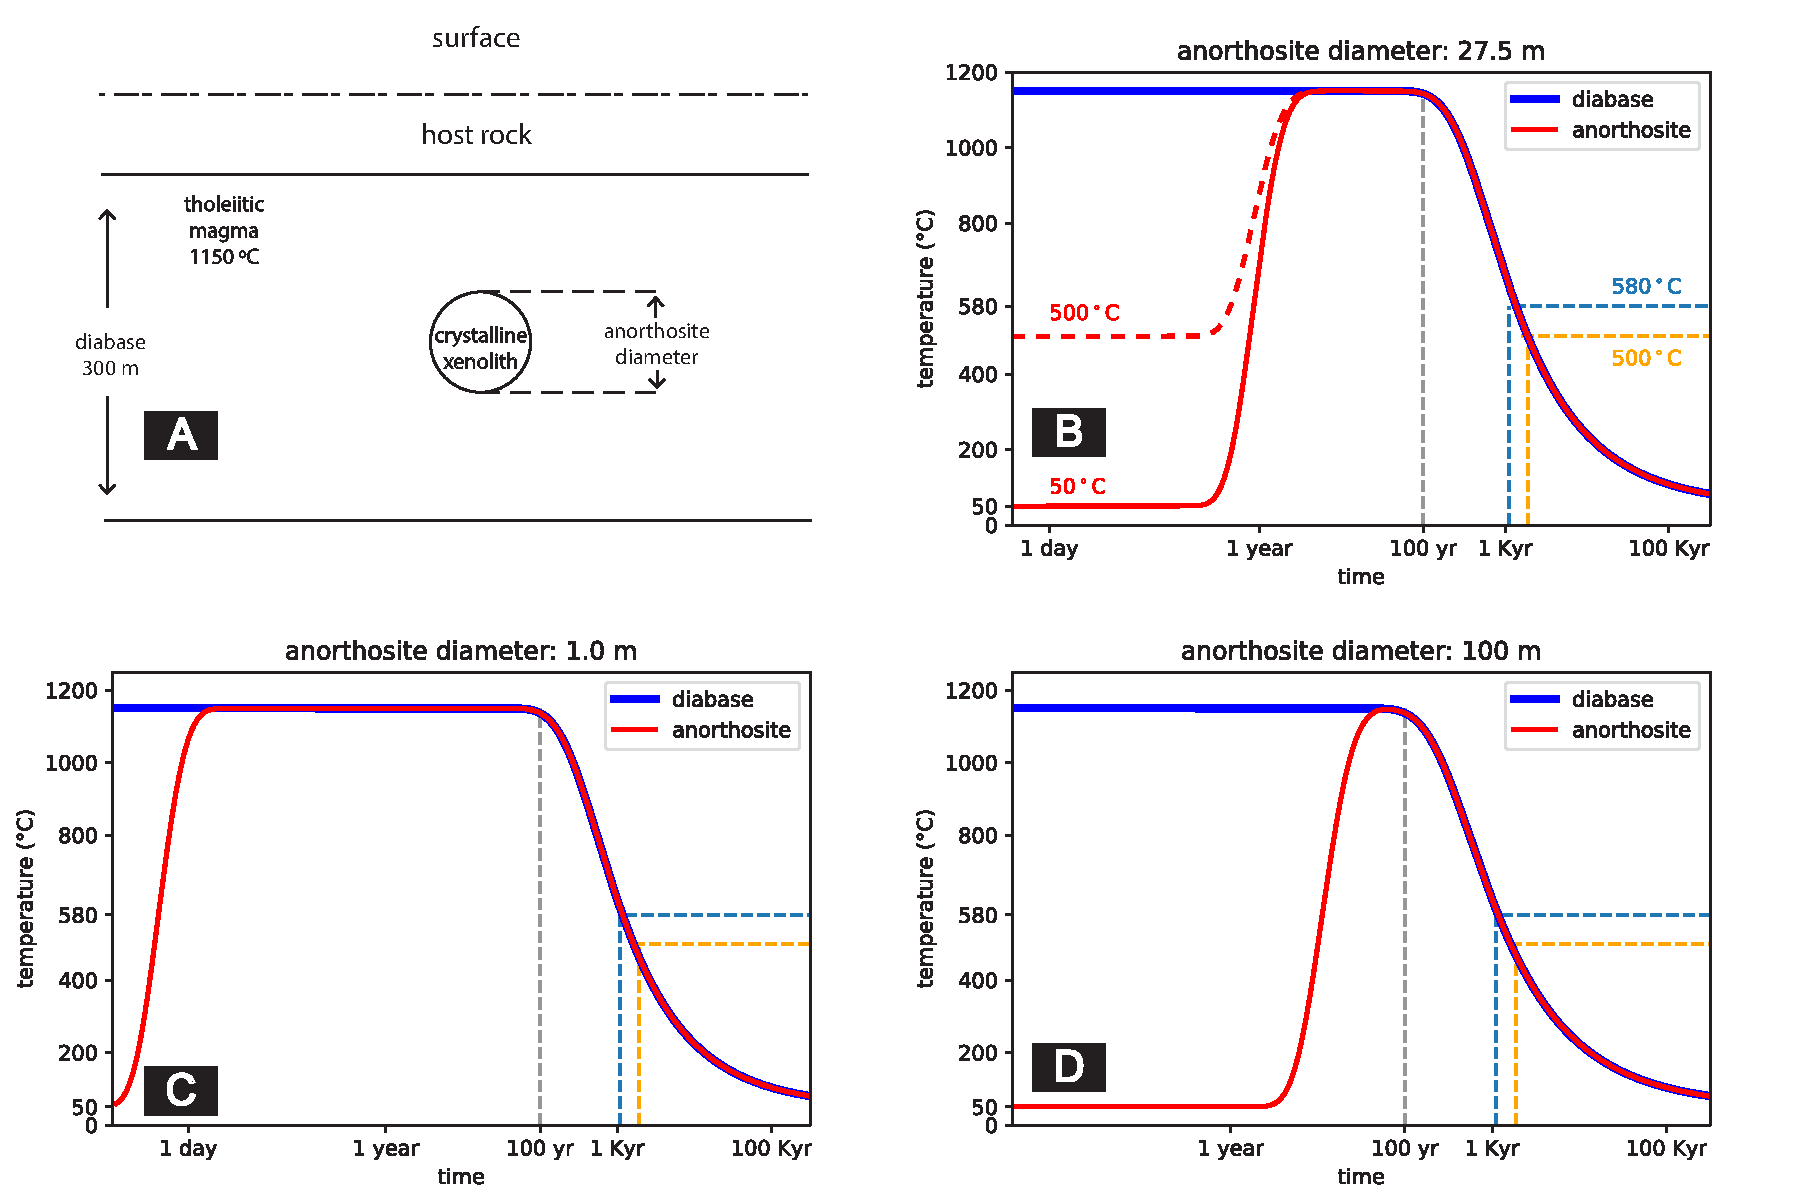
\includegraphics[width=\textwidth]{figure/Zhang2021/thermal_history_model.pdf}
\caption[Thermal history model of the Beaver River diabase and its anorthosite xenoliths after emplacement at hypabyssal depths.]{\footnotesize{Thermal history model of the Beaver River diabase and its anorthosite xenoliths after emplacement at hypabyssal depths. (A) Schematic diagram for the thermal model considering cool anorthosite xenoliths as crystalline spheres residing in the middle of a diabase sill. Together they are hosted by cool country rocks at shallow depths. (B) Specific model for anorthosite AX16 (diameter of 27.5 meters) within its diabase sill host which is estimated to be 323 meters thick. (C) Thermal history model considering an anorthosite xenolith 1 meter in diameter residing in a 300 meter diabase sill. (D) Thermal history model considering an anorthosite xenolith 100 meter in diameter residing in a 300 meter diabase sill. These models show that anorthosite xenoliths were heated up to the diabase melt temperature after the emplacement, regardless of size. The time elapsed between at magnetite blocking temperatures (580\textdegree C and 500\textdegree C) during cooling is on the scale of a thousand years.}}
\label{fig:thermal_history_model}
\end{figure}

The consistency of the paleomagnetic directions between the anorthosite xenoliths and the host diabase indicate that the anorthosites were heated above the Curie temperature of low-titanium titanomagnetite ($\sim$580\textdegree C) within the Beaver River diabase. To determine whether this thermal history is consistent with the geometry of the units and to gain more insight into the emplacement history of the xenoliths, we developed a cooling model. In this model, the anorthosite xenoliths are considered to be solid spheres with an initial cool temperature embedded in a uniform sheet of diabase magma \citep{Delaney1987a, Unsworth1979a}. The modeled thermal histories for various sizes of anorthosite xenoliths are shown in Fig. \ref{fig:thermal_history_model}. In one end member case, the initial temperature of the anorthosites is assumed to be 50\textdegree C. While this temperature is unrealistically low given that the anorthosites likely have a deep crustal source, thermal modeling shows that even a 100-meter anorthosite xenolith with such low initial temperature would have been heated to the temperature of the tholeiitic magma (1150\textdegree C) within the sill. This temperature is well above the Curie temperature of magnetite. Anorthosite xenoliths with an assumed initial temperature of 500\textdegree C will equilibrate with the magma temperature on a similar, but slightly shorter, timescale. Therefore, the model predicts that the remanent magnetizations of the anorthosites will be reset during emplacement within the diabase sills, regardless of their initial temperatures. Model parameters set to match the xenolith AX16, from which a U-Pb date was developed in this study, leads to a model where the 27.5 m xenolith would have stayed at the magma temperature for about 100 years after sill emplacement (Fig. \ref{fig:thermal_history_model}). This duration estimate is a minimum as it does not consider heating associated with melt in the lower crust or during ascent prior to emplacement although this was likely rapid. The xenolith would have then cooled through the Curie temperature of magnetite (580\textdegree) after $\sim$1 kyr and acquired its magnetization as it cooled through magnetite blocking temperatures (down to $\sim$500\textdegree, Fig \ref{fig:Demag}).

\section{Discussion}
\subsection{Origin and Age of the Anorthosite Xenoliths}

There have been divergent interpretations regarding the age and magma source of the anorthosite xenoliths in the Beaver River diabase (Fig. \ref{Chap_BBC_Geologic_map}). \cite{Grout1939a} recognized the xenolithic nature of the anorthosites and suggested that the massive intrusion of the older anorthositic gabbro within the Duluth Complex may have supplied anorthosite fragments that were later entrained by the Beaver River diabase emplacement. \cite{Morrison1983a}, on the other hand, argued that the xenoliths were sourced from Paleoproterozoic or Archean lower crust that were liberated and contaminated by Midcontinent Rift magmas based on Sm and Nd isotopic data. They interpreted a Sm-Nd model age of 1.9 Ga from one of the xenoliths as providing a minimum crystallization age for the anorthosites though they acknowledged that these constraints are not definitive with respect to the age. 

In contrast to this Archean to Paleoproterozoic model, \cite{Miller1997a} favored a scenario where the anorthosite crystallized as part of Midcontinent Rift magmatism. They cited work by \cite{Kushiro1980a} who showed that the changing density contrast between labradoritic to bytownitic plagioclase and tholeiitic magma at different crustal pressures would promote flotation of plagioclase in deep ($>$20 km) crustal magma chambers and the creation of anorthosite cumulates in the lower crust. This mechanism of plagioclase flotation likely created massive anorthosite cumulates in the roof zones of subcrustal magma chambers during MCR magmatism. \cite{Miller1990a} speculated that plagioclase-phyric magmas tapped from these deep chambers fed shallow ($\sim$5 km) subvolcanic intrusions of the Duluth Complex, thereby creating the troctolitic anorthosites and gabbroic anorthosites of the Anorthositic Series. \cite{Miller1997a} suggested that the nearly pure anorthosite xenoliths occurring in the younger and more hypabyssal diabase intrusions of the Beaver Bay Complex were harvested from these phase-segregated intrusions in the lower crust. They further argued that the isotopic data of \cite{Morrison1983a} can be explained by anorthosite-forming MCR magmas having been contaminated by older crust rather than the anorthosites being older lower crust that was contaminated by MCR magmas.

Our new geochronology documents that the anorthosite xenoliths were liberated from depth and were emplaced within the shallow intrusions of the Beaver River diabase at 1091.7 $\pm$ 0.2 Ma (95\% CI). This timing of emplacement is constrained by the Beaver River diabase postdating the new $^{206}$Pb/$^{238}$U zircon date of 1091.83 $\pm$ 0.21 Ma for the AX16 xenolith and being older than the cross-cutting 1091.61 $\pm$ 0.14 Ma Silver Bay intrusives.

The most straight-forward interpretation of the anorthosite 1091.83 $\pm$ 0.21 Ma U-Pb zircon dates is that they record crystallization of the anorthosite cumulates during Beaver Bay Complex magmatism just before the time of Beaver River diabase emplacement. The significant negative Eu anomaly in the zircons within the anorthosite constrains them to have crystallized from a magma that had experienced significant plagioclase extraction (Fig. \ref{fig:REE}; \citealp{Rubatto2002a, Schaltegger1999a}). This result indicates that the zircons were comagmatic with their host anorthosite plagioclase. The Ti-in-zircon temperature estimates indicate that they crystallized from temperatures of $\sim$998 to 860\textdegree C (Supporting Information; \citealp{Ferry2007a}). In addition, zircons that have lower Ti-in-zircon temperatures have lower Eu abundance, but enrichment of incompatible elements such as Hf and Th (Supporting Information). This systematic pattern of elemental concentration variation is consistent with the zircons crystallizing from residual melts on a cooling path that increased incorporation of incompatible trace elements and deepened the Eu anomaly with decreasing temperature and melt fraction. Scanning electron microscopy on two undated anorthosite xenoliths with plagioclase laths displaying interlocking textures shows zircon crystals with subhedral to anhedral shapes within the mineral assemblage that is interstitial to the plagioclase (Supporting Information). Cathodoluminescence (CL) images show internal zoning in zircons which can be attributed to variations in REE, particularly Dy elemental concentrations, during zircon crystallization (Fig. \ref{fig:CL_image}; \cite{Remond1992a}). These data confirm that the zircons formed from residual melt within the interstitial spaces of the plagioclase cumulate and are inconsistent with a later metamorphic origin.

This scenario requires that there were large lower crustal magma chambers in which flotation of plagioclase resulted in cumulate formation during ca. 1092 Ma Beaver Bay Complex magmatism and contrasts with the model of \cite{Miller1997a} for an older origin of the anorthosite during the ca. 1096 Ma Duluth Complex magmatism. Zircon U-Pb dates nearly always record crystallization age as the temperatures necessary for significant diffusive Pb loss exceed typical liquidus temperatures of zircon-bearing rocks. However, the anorthosites are a rather unique case given that the melting point of anhydrous plagioclase with an average composition of the Beaver River anorthosite ($\sim$70$\%$ anorthite; \citealp{Morrison1983a, Doyle2016a}) is quite high at $\sim$1400\textdegree C. Thermal modeling indicates that the xenoliths would have equilibrated to the temperature of the olivine tholeiitic magma ($\sim$1100 to 1200\textdegree C) and remained at that temperature for more than 100 years in the diabase sill interior (Fig. \ref{fig:thermal_history_model}). While these temperatures would not have melted the plagioclase or zircon, they are high enough to consider the possibility of Pb diffusion out of zircon. Could diffusive resetting of the zircon in the anorthosite cumulates xenoliths allow their crystallization at ca. 1096 Ma in the deep crust, but the closure of U-Pb zircon chronometer upon emplacement and cooling at ca. 1091.8 Ma?

\begin{figure}[h!]
\noindent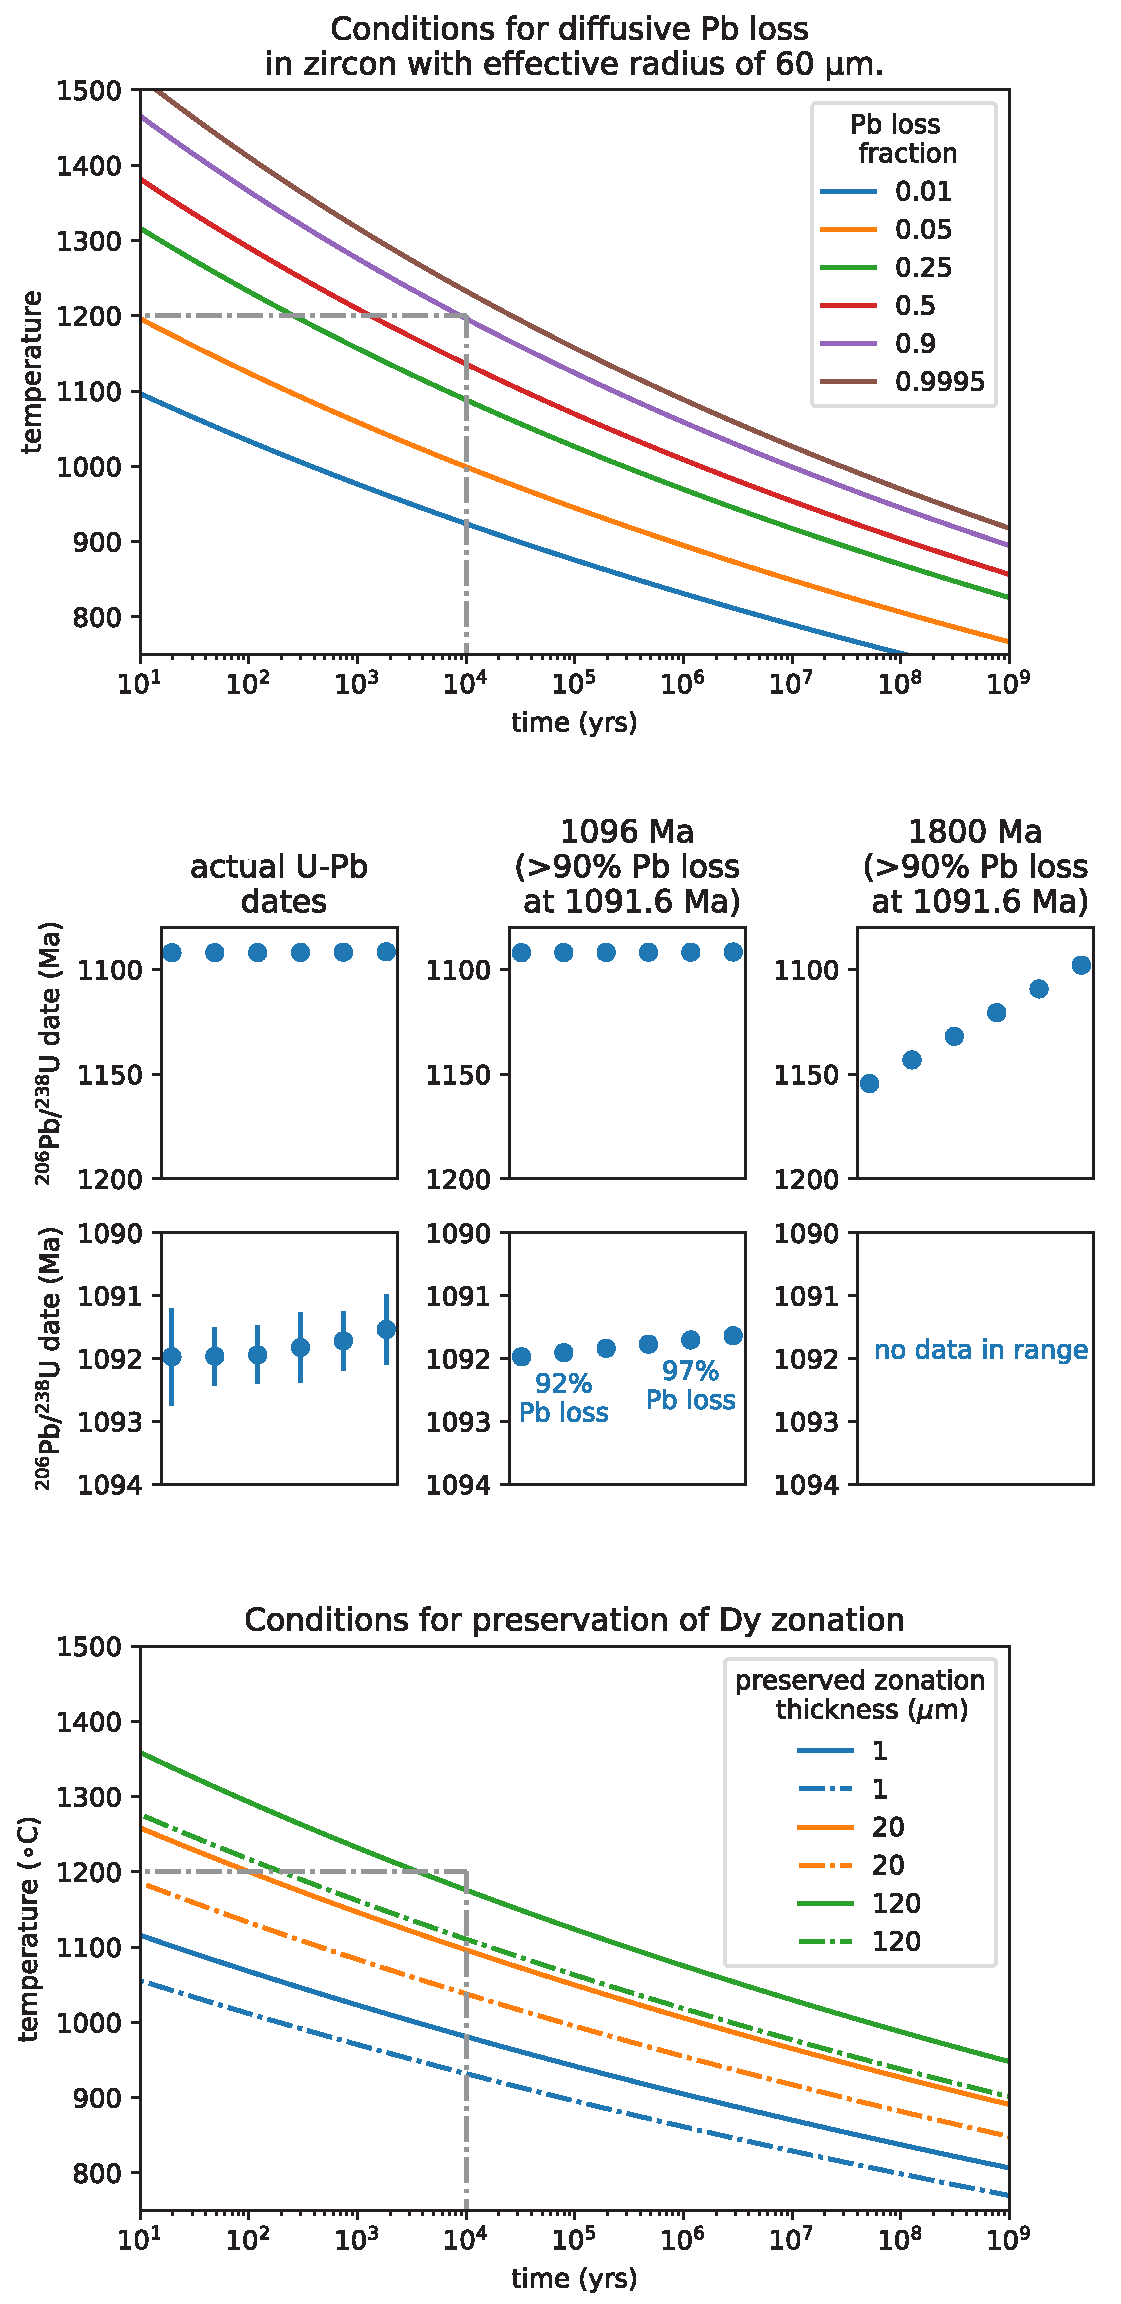
\includegraphics[width=0.47\textwidth]{figure/Zhang2021/diffusive_loss.pdf}
\centering
\caption[Zircon diffusion modeling]{\footnotesize{Top: Conditions for diffusive Pb loss in crystalline zircon for zircons of effective radii of 60 $\mu$m. Curves represent time--temperature conditions under which zircon will lose the indicated fraction of total Pb. Middle: Modeled zircon Pb loss scenarios with initial crystallization ages of 1091.8 Ma, 1096 Ma, and 1800 Ma with varying degrees of Pb loss at 1091.6 Ma compared to the actual U-Pb dates. Bottom: Conditions for preservation of Dy zoning in zircon. Curves represent time-temperature conditions under which different zoning thicknesses would be preserved in zircon. For conditions above the upper solid curves in each group, well-defined zoning will be lost at a given thickness. For conditions above the dashdot lines, zones will be partially lost but will retain initial composition in zone center. Pb diffusion and Dy zoning models follow \cite{Cherniak2001a} and \cite{Cherniak1997a}.}}
\label{fig:diffusive_loss}
\end{figure}

The magnitude of Pb diffusion is dependent on the time spent at such a temperature. Using the diffusion parameters of \cite{Cherniak2001a}, a sustained temperature of 1200\textdegree C for $\sim$10 thousand years is required for diffusive loss of $\sim$90\% of Pb from a $\sim$120 $\mu$m diameter zircon. In this case, zircons that crystallized at 1096 Ma and then lost $>$90\% of their Pb at 1091.6 Ma could give apparent U-Pb dates of 1091.8 Ma that are reproducible at the measurement resolution (Fig. \ref{fig:diffusive_loss}). However, CL imagery reveals sharp boundaries between zones of differing CL response (Fig. \ref{fig:CL_image}) on the scale of $\sim$2 $\mu$m. Such CL zoning patterns are dominantly attributed to concentration variations in the rare earth element Dy \citep{Remond1992a}. A time-temperature history that results in 90\% Pb diffusion out of a 120 $\mu$m diameter zircon would also cause Dy re-equilibration throughout a zircon, leaving no clear zonation (Fig. \ref{fig:diffusive_loss}; \citealp{Cherniak1997a}). Therefore, a scenario where the zircons first crystallized during Duluth Complex magmatism and subsequently lost more than 90\% of Pb is exceedingly difficult to reconcile with the preservation of such thin, sharp zones. In fact, preservation of REE zoning in these zircons limits heating at the emplacement temperatures of the Beaver River diabase to a duration more consistent with our modeled duration of $\sim$100 years of heating prior to cooling to the temperatures that preserve such zonation (Fig. \ref{fig:thermal_history_model}, \ref{fig:diffusive_loss}). It is therefore most probable that the Beaver River diabase anorthosite xenoliths are entrained cumulate enclaves that formed at the time of Beaver Bay Complex magmatism. 

\subsection{A comagmatic relationship between the Beaver River diabase and the Greenstone Flow}

Given the existence of many anorthosite xenoliths whose short-axis diameters often reach tens of meters and can be as wide as 180 meters (Fig. \ref{Chap_BBC_Geologic_map}; \citealp{Boerboom2004a, Boerboom2006b}), the Beaver River diabase magma conduits must have been at least this wide during magma ascent. It would be consistent with such wide conduits extending to hypabyssal depths for magma that flowed through these conduits to have vented to the surface.
 
 \begin{figure}[h!]
\centering
\noindent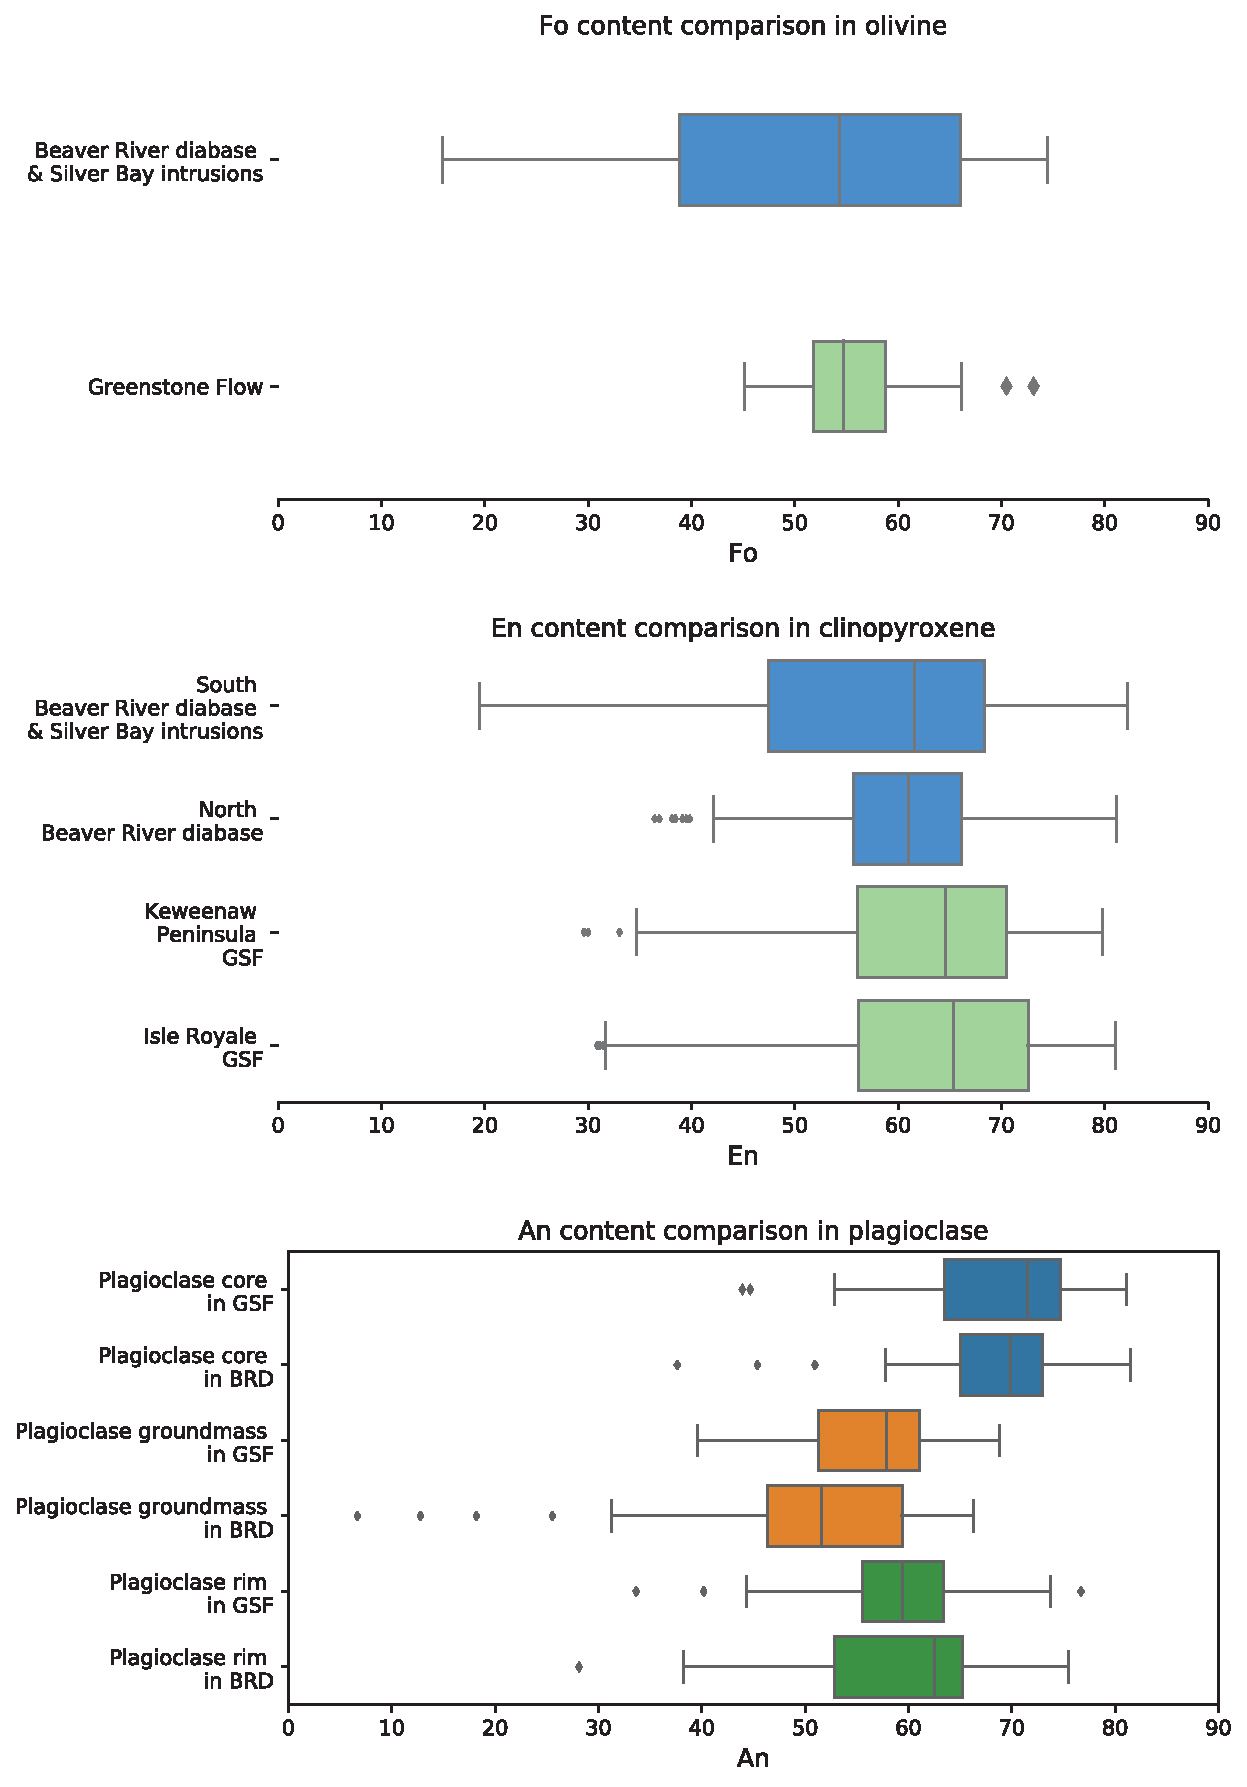
\includegraphics[width=0.68\textwidth]{figure/Zhang2021/Geochem.pdf}
\caption[Box plots of geochemical analyses of olivine, pyroxene, and plagioclase in the Beaver River diabase (BRD) and Greenstone Flow (GSF).]{\footnotesize{Box plots of geochemical analyses of olivine, pyroxene, and plagioclase in the Beaver River diabase (BRD) and Greenstone Flow (GSF). The forsterite content in olivine crystals and the enstatite content in clinopyroxene crystals are very similar in the Beaver River diabase and the Greenstone Flow. The anorthite concentrations in the core, groundmass, and rim of the plagioclase megacrysts within the Beaver River diabase and the Greenstone Flow share very similar patterns and the distributions are nearly identical. The box encloses the middle 50\% of the data ranges (i.e., the interquartile range), and the notch represents the median values. The whiskers extend to the 2.5th and 97.5th percentile values. Fo-forsterite; En-enstatite; An-anorthite. Data from \cite{Doyle2016a}.}}
\label{fig:Geochem}
\end{figure}

The high volume of the extrusive Greenstone Flow of the Portage Lake Volcanics lead to a potential match for this large feeder system. \cite{Doyle2016a} proposed a comagmatic link between the Beaver River diabase and the Greenstone Flow. \cite{Doyle2016a} discovered that both the intrusive Beaver River diabase and the Greenstone Flow have indistinguishable primary compositions that followed similar differentiation patterns. \cite{Doyle2016a} also highlighted the shared petrographic textures between the ophitic Beaver River diabase and the ophitic Greenstone Flow, which features the plagioclase laths clustering together and joining along their long crystallographic axes. The forsterite content of the olivines and enstatite content of the pyroxenes in the Beaver River diabase together with the Silver Bay intrusions, and the Greenstone Flow have overlapping compositions consistent with the same magma source (Fig. \ref{fig:Geochem}). The composition of the plagioclase within the units further strengthens this interpretation. Although there are no known multi-crystalline anorthosite xenoliths in the Greenstone Flow, plagioclase megacrysts occur in the lava flow. Analyses of the anorthite content from plagioclase megacrysts show very similar values between the Beaver River diabase and the Greenstone Flow basalt (Fig. \ref{fig:Geochem}; \citealp{Doyle2016a}). In both units, the plagioclase cores are more enriched in anorthite than the rim and the groundmass. These data provide evidence that the core of the plagioclase megacrysts in the Greenstone Flow derived from a similar source with those in the Beaver River diabase and that the rims are later overgrowths. These mineralogical similarities are consistent with the interpretation that the Beaver River diabase and the Greenstone Flow have the same magma source. 


The synchroneity between the Beaver River diabase and the Greenstone Flow inferred from comparable lithologies and geochemistry can be further evaluated using the paleomagnetic pole positions and radioisotopic dates from both units (Fig. \ref{fig:Direction_pairs}, \ref{fig:BBC_geochron}). The heat diffusion model of the cooling history of the anorthosite xenoliths within the diabase suggests that the time it takes to cool the diabase and anorthosite from low-titanium titanomagnetite Curie temperature ($\sim$580\textdegree C) to their blocking temperatures ($\sim$500\textdegree C) is on the time scale of a few thousand years (Fig. \ref{fig:thermal_history_model}). This time scale is close to the typical 10$^4$ years which is considered to be sufficient for averaging out secular variations of the geomagnetic field. Fig. \ref{fig:Direction_pairs} shows the site mean paleomagnetic pole positions from all diabase and anorthosite sites in this study against the previously synthesized Laurentia APWP developed using an Euler pole inversion to chronostratigraphically constrained volcanic poles in present-day coordinates \citep{Swanson-Hysell2019a}. The site-mean pole positions of the diabase and anorthosite overlap within uncertainty ellipses and the mean pole positions fall between the 1095 Ma and 1090 Ma pole path positions (Fig. \ref{fig:Direction_pairs}), consistent with the geochronology results (Fig. \ref{fig:BBC_geochron}). Further, the mean paleomagnetic pole position derived from the Greenstone Flow share a common mean with those of the Beaver River diabase and the anorthosite xenoliths, but these poles do not share a common mean with the mean pole derived from the Portage Lake Volcanics (Fig. \ref{fig:Direction_pairs}; \citealp{Swanson-Hysell2019a}). This result suggests that the timescale over which the Beaver River diabase and the Greenstone Flow acquired their magnetization may be too short to fully average out secular variation. In this case, the overlapping pole positions between the Beaver River diabase and the Greenstone Flow strengthens their temporal correlation even more (Fig. \ref{fig:Direction_pairs}). 

\begin{figure}[h!]
\centering
\noindent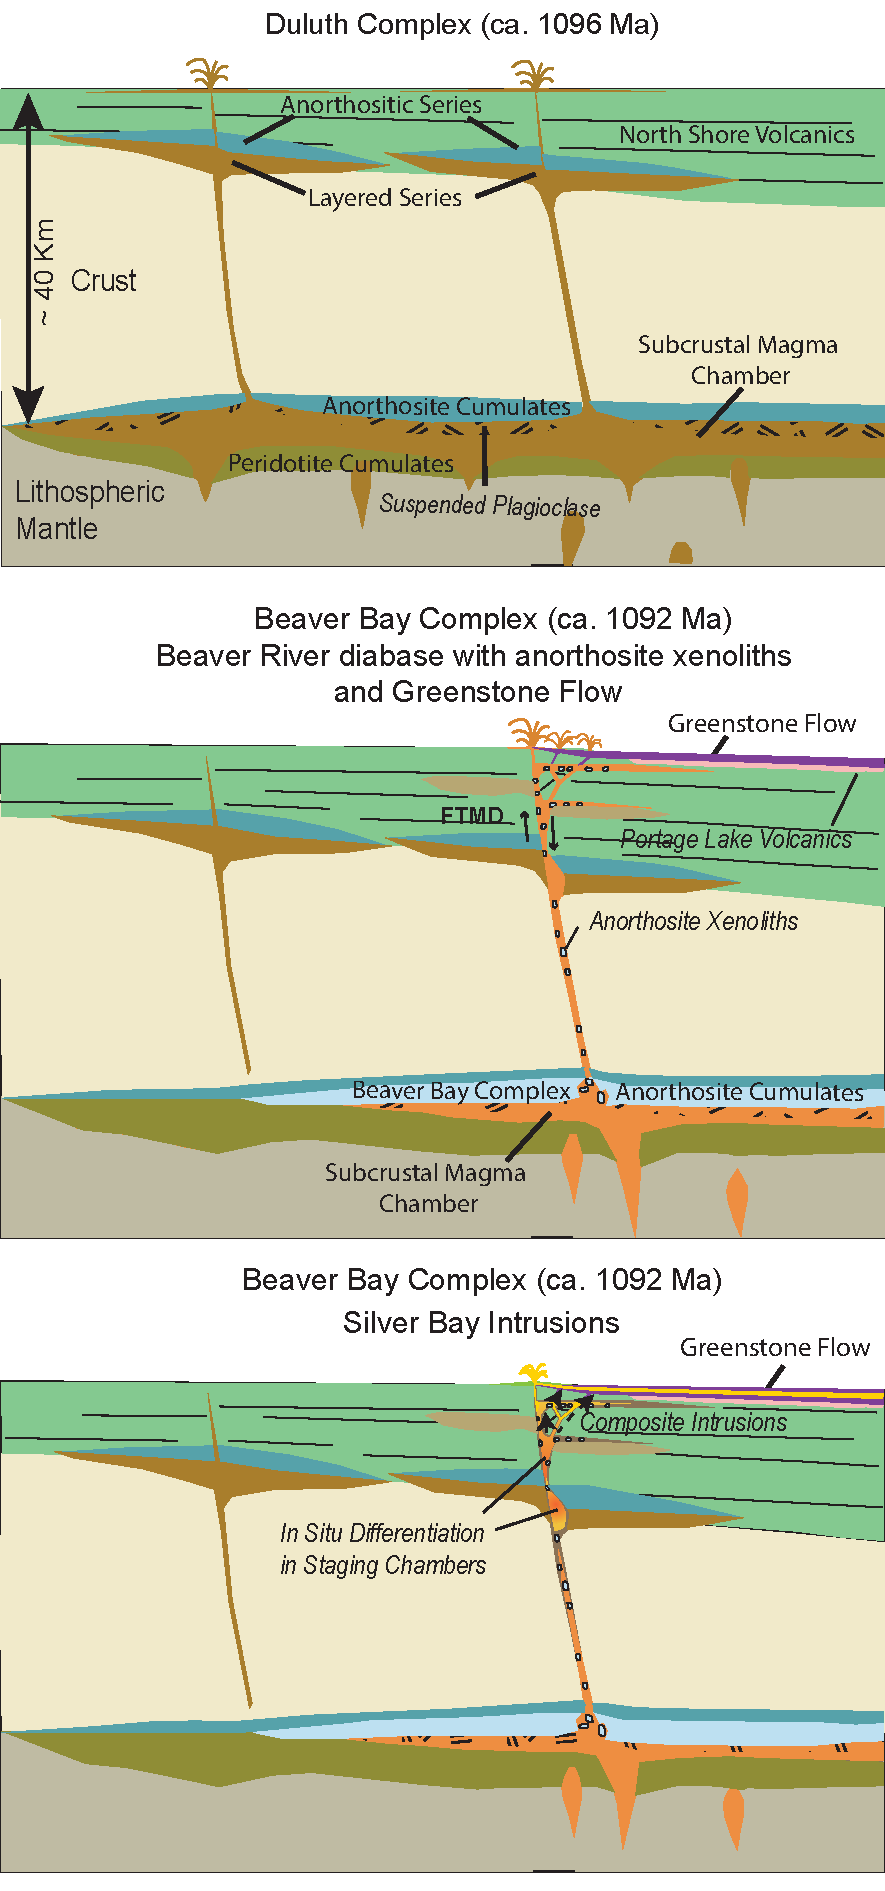
\includegraphics[width=0.4\textwidth]{figure/Zhang2021/Flank_eruption.pdf}
\caption[Schematic illustration of the emplacement of the ca. 1096 Ma Duluth Complex, the ca. 1092 Ma Beaver Bay Complex, Greenstone Flow and associated anorthositic lithologies]{\footnotesize{Schematic illustration of the emplacement of the ca. 1096 Ma Duluth Complex, the ca. 1092 Ma Beaver Bay Complex, Greenstone Flow and associated anorthositic lithologies. Top: Duluth Complex Anorthositic Series formed by subhorizontal emplacement of plagioclase crystal mushes generated by plagioclase flotation in subcrustal magma chambers. The Layered Series formed by emplacement of crystal-poor mafic magmas beneath the Anorthositic Series and variable differentiation by in situ fractional crystallization. Middle: Development of a deep crustal magma chamber that formed anorthosite cumulates and intrusion of the anorthosite xenolith-bearing Beaver River diabase of the Beaver Bay Complex along a major crustal fault (FTMD-Finland Tectonomagmatic Discontinuity) and its massive eruption at surface that could have formed the Greenstone Flow. Bottom: Emplacement of the Beaver River diabase and the Greenstone Flow. The Silver Bay intrusion may have added to the composite composition of both units, through magma differentiation in deeper staging chambers. The erosional unconformity between the Schroeder-Lutsen basalt and the Beaver River diabase suggest the diabase was emplaced into an uplifted rift flank highland which would have led to flank eruptions into the main Midcontinent Rift basin.}}
\label{fig:Flank_eruption}
\end{figure}

The U-Pb dates are consistent with a comagmatic relationship as they reveal indistinguishable ages for the Beaver River diabase and the Greenstone Flow. The age of the Beaver River diabase is constrained to be between the $^{206}$Pb/$^{238}$U dates of  1091.83 $\pm$ 0.21 Ma and 1091.61 $\pm$ 0.14 Ma (Fig. \ref{fig:BBC_geochron}) giving an age estimate of 1091.7 $\pm$ 0.2 Ma (95\% CI). This age is indistinguishable with the $^{206}$Pb/$^{238}$U date of 1091.59 $\pm$ 0.27 Ma for the Greenstone Flow (Fig. \ref{fig:BBC_geochron}).

The Portage Lake Volcanics, including the Greenstone Flow, are interpreted to have erupted into the main central graben of the Midcontinent Rift during an interval of significant subsidence (Fig. \ref{fig:Flank_eruption}; \citealp{Miller1997a,Cannon1992b}). In contrast to the thick accumulation in the Portage Lake Volcanics, the Beaver Bay Complex has an erosional (and slightly angular) unconformity atop it that is then covered by the younger Schroeder-Lutsen basalt (Fig. \ref{Chap_BBC_Geologic_map}; \cite{Miller2001a}). This relationship suggests that the Beaver River diabase was emplaced into a rift flank highland that experienced uplift during the active development of the central graben \citep{Swanson-Hysell2019a}. Eruptions fed through the Beaver River diabase network would have emerged from the rift flank and flowed from the highland into main rift basin (Fig. \ref{fig:Flank_eruption}). 

The proposed intrusive-extrusive connection between the Beaver River diabase and the Greenstone Flow would imply that the Greenstone Flow extended for more than 250 km from northeastern Minnesota to the northern end of Isle Royale where the flow is $\sim$100 m thick and to the northeastern end of the Keweenaw Peninsula, where the flow is $\sim$400 m thick (Fig. \ref{Chap_BBC_Geologic_map}). With this length, the full volume of the Greenstone Flow reaches $\sim$6000 km$^3$ \citep{Doyle2016a}, rivaling the largest known lava flows on Earth (Fig. \ref{fig:lava_flow_rank}). Such lengths were achieved for multiple high volume flows within the Columbia River basalts \citep{Reidel2013a} and are modest compared to the Rajahmundry Trap lavas of the Deccan Traps which traveled $\sim$1000 km \citep{Self2008a}. One potential challenge for a flow having traveled from the Beaver River diabase to the Portage Lake Volcanics is that a reconstruction of present-day rift basin isopachs from seismic data indicates that there is a deep bowl-shaped volcanics-filled basin offshore of Minnesota and the Beaver Bay Complex \citep{Stewart2018a}. While this basin has a thicker accumulation of volcanics than surrounding regions, it is unclear whether it was a topographic barrier. If it was, it could have prevented lavas from present-day northern Minnesota from reaching the portion of the basin now exposed on the Keweenaw Peninsula. Therefore, it is also possible that the indistinguishable ages and similar geochemistry between the Beaver River diabase and the Greenstone Flow are the result of them having been derived from a contemporaneous deep magmatic source without being connected on the surface. 

\section{Conclusion}

There was voluminous emplacement of magma into the shallow subsurface and eruption into the Midcontinent Rift basin ca. 1091.7 Ma at the end of the main stage of Midcontinent Rift volcanism. The anorthosite xenoliths within the Beaver River diabase and their U-Pb geochronology, whose interpretation is informed by REE patterns, indicate that there was a contemporaneous deep crustal magmatic system in which flotation of plagioclase formed anorthosite cumulates. The large dimension of the anorthosite xenoliths require that conduits feeding magma to the surface had widths that exceeded 150 meters. These conduits would have delivered a high volume of magma into the rift basin. The high-precision U-Pb dates, together with paleomagnetic and geochemical data, are consistent with the hypothesis that the Beaver River diabase was the  feeder system of the Greenstone Flow although they could have been disconnected at the surface and both be emblematic of this high-volume pulse of magmatism..

\section{Acknowledgments}
Project research was supported by NSF CAREER grant EAR-1847277 to Nicholas L. Swanson-Hysell and an Institute on Lake Superior Geology Student Research Fund grant to Yiming Zhang. Permits for fieldwork and sampling from the Minnesota Department of Natural Resources are gratefully acknowledged. The authors thank James Pierce and Blake Hodgin for assistance in the field. The authors thank Stephen Self for providing constructive comments regarding mafic lava flow volumes. We thank John Grimsich and Tim Teague at UC Berkeley EPS department for their help with petrographic sample preparation and analyses. We thank U.S. Geological Survey reviewer Jonathan Hagstrum and journal reviewers Bernie Housen and William Rose for their constructive comments on the manuscript.
